% Preserve searchable text, including ligatures, in the compiled PDF.
\RequirePackage{cmap}
\documentclass[preprint,12pt]{elsarticle}

\usepackage{amsmath,amssymb,amsfonts}
\usepackage{graphicx}
\usepackage{booktabs}
\usepackage{multirow}
\usepackage{xurl}
\usepackage{xcolor}
\usepackage[hidelinks,hypertexnames=false]{hyperref}
\hypersetup{pdfauthor={Paolo Grazieschi, Romeo Silvestri, Massimo Vecchio, Mattia Antonini, Fabio Antonelli}}

\usepackage{longtable}
\setlength{\LTcapwidth}{\textwidth}

\journal{Knowledge-Based Systems}

\setlength{\emergencystretch}{2em}
\begin{document}

\begin{frontmatter}

\title{Residual Drift Detectors under a Common False-Alarm Budget: A Calibrated Comparison with a Wasserstein Detector}

\author[fbk]{Paolo Grazieschi\corref{cor1}}
\ead{pgrazieschi@fbk.eu}
\cortext[cor1]{Corresponding author.}

\author[fbk]{Romeo Silvestri}
\ead{rsilvestri@fbk.eu}

\author[fbk]{Massimo Vecchio}
\ead{mvecchio@fbk.eu}

\author[fbk]{Mattia Antonini}
\ead{m.antonini@fbk.eu}

\author[fbk]{Fabio Antonelli}
\ead{fantonelli@fbk.eu}

\affiliation[fbk]{organization={OpenIoT Research Unit, Fondazione Bruno Kessler}, addressline={Via Sommarive 18}, postcode={38123}, city={Trento}, country={Italy}}

\begin{abstract}
Comparing drift detectors for deployed regression models requires accounting for differences in false-alarm rates. We compare ADWIN, KSWIN, Page-Hinkley and a calibrated Wasserstein detector under a common false-alarm budget, calibrating each on drift-free streams and auditing it on held-out null streams. The Wasserstein detector monitors squared residuals by combining the empirical $1$-Wasserstein distance, a rolling interquartile-range score and hysteresis. Across seven abrupt synthetic change scenarios, it alone detects $96$-$100$\% of changes in every scenario. Each baseline falls to placebo level in one scenario targeting a known weakness of its statistic: ADWIN and Page-Hinkley on a noise change that preserves the mean squared error, and KSWIN on large errors confined to a small fraction of inputs. All detectors detect at least $94$\% of changes in the other five. The baselines are faster: ADWIN on most functional changes and KSWIN on the mean-preserving noise change, whose weaker versions it also detects at least as often. In an illustrative soil-moisture case with an upstream model upgrade, Wasserstein raises the fewest alarms and stays within budget, at the same rate as on a control target; its rolling reference adapts to a slow, months-long rise in residuals at one site, which suggests pairing it with a fixed-reference level check. These results support distributional monitoring for changes that preserve the mean of the monitored signal, and the Wasserstein distance for changes that move a small share of residual mass far.
\end{abstract}
\begin{highlights}
\item Drift detectors for regression compared under one calibrated false-alarm budget
\item Calibration on drift-free streams; audit on held-out null streams
\item Each baseline falls to placebo on a change its test statistic cannot see
\item Wasserstein detector finds 96--100\% of changes in all seven synthetic scenarios
\item Real soil-moisture case shows how budget and rolling reference shape alarms
\end{highlights}
\begin{keyword}
Concept drift \sep drift detection in regression \sep false-alarm control \sep Wasserstein distance \sep data streams
\end{keyword}
\end{frontmatter}

\section{Introduction}
\label{sec:intro}
Prediction systems for demand forecasting, industrial monitoring and agriculture rely on relationships learned from historical data~\cite{douaioui2024machine,Ge2017DataMA,grazieschi2025soilcast}. When those relationships change, or when the noise around them does, a deployed model starts to make errors of a different size or shape. This is why MLOps pipelines include post-deployment stages~\cite{antonini2022tiny} in which the model is watched after its initial evaluation, and an alarm is raised when anomalies are detected. This alarm can prompt an investigation, a recalibration of predictive uncertainty or retraining. Such a warning component is useful only if it catches the relevant changes without alarming too often when nothing has changed.

Prediction errors are a natural interface between a model and its monitor. Once the target is observed, the error can be passed to a univariate detector that knows nothing about the model's internals. The price is that targets must be available. Watching errors also brings out a distinction that is easy to blur: the distribution of error magnitudes can change while the expected squared loss stays the same, and a running average of the error would then miss the change.

A sensitive distributional statistic is only part of a detector. On its own it does not say how often the detector will alarm, and a short delay on the streams where a change was found can hide the streams where it was missed. We combine three established pieces. The empirical $1$-Wasserstein distance compares older and recent squared residuals. A rolling quartile-based score measures how unusual the current distance is compared with its recent history. Hysteresis then emits one alarm per excursion and re-arms only when the score returns to its baseline region. The operating point is chosen offline, on drift-free streams, under a declared false-alarm budget.

The question behind the comparison is when a distributional statistic is the better choice. For any transform of the residual that a monitor might track, some changes leave its mean in place and move its higher moments; a detector that follows the mean of that signal cannot see them, whereas a detector that compares whole distributions can. Among distributional statistics, the Wasserstein distance grows with how far the affected probability mass moves, while the Kolmogorov-Smirnov distance is capped by how much mass moves (Section~\ref{sec:method}). We therefore expect the Wasserstein detector to be preferable when a change may leave the mean of the monitored signal unchanged or move a small share of the errors far, and Kolmogorov-Smirnov-type tests to be at least as good for changes in the shape of the bulk of the distribution. The experiments test these expectations on abrupt synthetic changes.

We evaluate coverage, delay and alarm volume on separate drift and held-out null streams. The synthetic benchmark contains abrupt functional changes and a switch from Gaussian to bimodal noise that keeps the mean and variance of the noise. The Wasserstein detector is the only one that finds most changes in every scenario: in five scenarios every detector finds at least 94\% of the changes, and in each of the other two, built around a known limitation of one statistic, a baseline misses almost all of them. The baselines lead on speed: ADWIN usually reacts sooner to functional drift, and KSWIN to the bimodal change, which it also detects at least as often at weaker separations. We also study repeated calibration and residuals that arrive in batches. Finally, we run the four detectors on a real soil-moisture forecaster whose target changed when the upstream data provider upgraded its model (Section~\ref{sec:soil}), to see how the machinery around the statistic, a rolling reference and a strict budget, behaves on slowly changing real residuals.

The contributions are:
\begin{enumerate}
\item A comparison of ADWIN, KSWIN, Page-Hinkley and a calibrated Wasserstein detector under the same shared protocol on seven abrupt synthetic scenarios, together with an explanation of where each statistic is blind: mean-based detectors cannot see changes that preserve the mean of the monitored signal, and the Kolmogorov-Smirnov distance is bounded by the fraction of mass that a local change moves.
\item A shared protocol that transfers the false-alarm matching of control charts to residual drift detectors with different statistics and parameters: each detector is tuned to a common false-alarm budget on drift-free streams, audited on held-out null streams and compared with a placebo rate, using a finite detection horizon, capped delays and paired statistical tests.
\item A specification of the calibrated Wasserstein detector, combining a distributional statistic, an adaptive score and an alarm state, and an assessment of these choices through separately calibrated ablations, sensitivity sweeps, repeated calibration draws and batch-end testing.
\item An illustrative application to day-ahead soil-moisture forecasts, in which a documented upgrade of an upstream data product provides a real change with a known date.
\end{enumerate}

\section{Related Work}
\label{sec:related}
Concept drift is a change in the data-generating process that can invalidate a learned predictor~\cite{gama2004,webb2016,lu2018,hovakimyan2024}; the dataset-shift literature describes the same problem from the point of view of a fixed model~\cite{QuioneroCandela2009DatasetSI}. A detector can watch the covariates, the predictions or the prediction errors, and each choice exposes different changes. We watch the squared errors of a fixed regression model. This requires observed targets and leaves some changes in the joint distribution of inputs and targets out of sight.

\paragraph{Error-based streaming detectors} Supervised detectors monitor a statistic of the predictor's errors. DDM tracks a binary classification-error indicator~\cite{gama2004}, so using it for regression would need an extra rule to turn a real-valued error into a binary outcome. Later error-based detectors keep this setting: STEPD compares recent and overall accuracy with a test of proportions~\cite{nishida2007stepd}, FHDDM bounds the drop of a sliding-window accuracy with Hoeffding's inequality~\cite{pesaranghader2016fhddm}, and the HDDM detectors apply Hoeffding-type bounds to moving averages of an input whose range is known in advance~\cite{frias2015hddm}; surveys review these and many other detectors~\cite{gama2014survey,lu2018}. Squared regression errors are neither binary nor bounded, so we do not include these detectors. ADWIN, KSWIN and Page-Hinkley, in the implementations used here, accept any univariate numeric stream~\cite{bifet2007,raab2020,page1954,hinkley1971}. ADWIN compares means over candidate subwindows, Page-Hinkley accumulates deviations from a running mean, and KSWIN applies a Kolmogorov-Smirnov test~\cite{massey1951kolmogorov} between a reference sample and recent observations. Because all three are available in \texttt{river}~\cite{montiel2021}, they can read exactly the same residual stream as our detector. KSWIN shows that distributional sensitivity is not unique to the Wasserstein distance; it belongs to a broader family of windowed two-sample detectors that compare a reference window with a recent one through a distance between empirical distributions, as in the framework of Kifer et al.~\cite{kifer2004detecting} and the incremental Kolmogorov-Smirnov test of dos Reis et al.~\cite{dosreis2016fast}; our detector is another member of this family.

\paragraph{Statistical process control} Control charts offer the classical framing of the trade-off between false alarms and delay. CUSUM charts~\cite{page1954}, of which Page-Hinkley is a variant, and EWMA charts~\cite{roberts1959control} are designed by fixing the in-control average run length (ARL$_0$), the expected number of observations before a false alarm, and then comparing out-of-control run lengths~\cite{montgomery2019introduction}. Our false-alarm budget plays the role of ARL$_0$: under the homogeneous Poisson working model of Section~\ref{sec:calibration}, $0.1$ alarms per 1,000 samples corresponds to an ARL$_0$ of about 10,000 samples, and the delay after a change corresponds to the out-of-control run length. Unlike control charts on a parameter with a known in-control distribution, the detectors compared here work on overlapping windows with adaptive states, so we estimate their false-alarm rates empirically. We include no separate EWMA or dispersion chart: Page-Hinkley represents the CUSUM family, and a chart on the variance of the squared residuals would respond to the bimodal shift of our benchmark, which lowers that variance (Section~\ref{sec:scenarios}), but a chart on any finite set of moments of the monitored signal is blind to changes that preserve those moments; adding moments moves the blind spot of a moment-based detector without removing it (Section~\ref{sec:coverage}).

\paragraph{False-alarm control in drift monitoring} Several drift detectors and evaluation frameworks already treat false alarms as a quantity to control. ECDD~\cite{ross2012ewma} monitors a classifier's error indicator with an EWMA chart whose control limits are set to give a chosen ARL$_0$. Podkopaev and Ramdas~\cite{podkopaev2022tracking} test sequentially whether the risk of a deployed model has risen beyond a tolerance, using time-uniform confidence sequences so that continuous monitoring does not inflate the false-alarm rate. CD-MOA~\cite{bifet2013cdmoa} evaluates change detectors on synthetic streams by their mean time between false alarms, together with detection delay and missed detections. Comparative studies have found that detectors differ considerably in false alarms and missed detections, and not only in delay~\cite{gonccalves2014comparative,barros2018large}, and Poenaru-Olaru et al.~\cite{poenaru2022concept} evaluate detectors explicitly as alarm systems. Nonparametric sequential tests with a chosen in-control run length also exist outside drift detection. The change-point-model charts of Ross and Adams use Kolmogorov-Smirnov and Cram\'er-von Mises statistics with thresholds set by simulation to give a chosen ARL$_0$~\cite{ross2012cpm,ross2015cpm}; online kernel detectors have been calibrated to a chosen expected run length~\cite{cobb2022sequential}; and conformal test martingales bound the probability of a false alarm under exchangeability~\cite{vovk2003testing,volkhonskiy2017inductive}. ECDD, the sequential risk test and these methods control false alarms within a single statistic, while CD-MOA reports them next to delay for each detector's chosen settings. Our protocol has a different aim: rather than a guarantee for one detector, it carries the ARL$_0$ matching of control charts over to heterogeneous streaming detectors, applying one empirical calibration rule and one held-out audit to detectors with different statistics, parameters and alarm states, so that differences in coverage and delay are measured under a common ceiling on the calibration false-alarm rate.

\paragraph{Input-space and unsupervised detection} A complementary line of work monitors the input distribution and needs no targets at all. Kernel two-sample statistics such as the maximum mean discrepancy~\cite{gretton2012kernel}, often applied after dimensionality reduction~\cite{rabanser2019failing}, test for covariate shift, and Lukats et al.~\cite{lukats2025benchmark} benchmark fully unsupervised detectors on real-world streams. Cluster-aware methods target changes that an aggregate statistic can hide, by monitoring each cluster or concept of an unlabelled stream separately~\cite{zhao2024imbalancedcluster,zhang2026unbiasedcluster} or by combining metrics for mixed numerical and categorical attributes with adaptive ensembles~\cite{zhao2022heterogeneous}. The masking problem they address has a counterpart in residual monitoring, where a change that affects only a fraction of the residual distribution limits the Kolmogorov-Smirnov distance (Section~\ref{sec:method}).

Input-side methods can alarm before any target arrives and can say where in feature space a change occurred, but they cannot see a change in the conditional relationship under a fixed input distribution, which is what the Friedman function switches of Section~\ref{sec:scenarios} produce. Residual monitoring detects such changes but has to wait for targets, so the two approaches complement each other. Model-aware detectors instead use information from inside the monitored model, for instance through transfer learning~\cite{wang2023model} or novelty detection on neural networks~\cite{shang2025novelty}. Since these families need different information, we restrict the comparison to detectors that treat the predictor as a black box and read the same scalar error stream.

\paragraph{Wasserstein and optimal-transport methods} The Wasserstein distance compares distributions through the cost of transporting one onto the other~\cite{villani2008}. It has been used to learn drift-invariant features for electronic noses~\cite{tao2019} and to detect drift in semiconductor manufacturing~\cite{lin2025}, and open-source monitoring tools report it as a data-drift measure~\cite{muller2024}. WATCH~\cite{faber2021watch} uses it for unsupervised change-point detection in multivariate time series. It compares each new mini-batch with a stored reference set through an approximate Wasserstein distance, signals a change when the distance exceeds a multiple of the largest distance seen within the reference, and then replaces the reference. Our detector applies a related comparison to a univariate error stream, calibrates its threshold to a declared false-alarm budget instead of a tuned ratio, and keeps its reference updating continuously, with hysteresis in place of a reset. Two further works monitor model outputs or errors. Laha and Verma~\cite{laha2021optimal} propose an optimal-transport drift detector for classifiers on sensor streams that summarises class-probability outputs over successive windows by Wasserstein barycentres and tests their divergence from a reference barycentre against a data-driven threshold. Wang et al.~\cite{wang2026dualchannel} monitor the residuals of a regression model through two channels: one filters point outliers, and the other diagnoses drift from an exponentially weighted moving absolute deviation, with dynamic thresholds that separate abrupt from incremental drift. Our detector also works on regression errors, but it compares empirical distributions of squared residuals with a two-sample distance; squaring keeps the magnitude of an error and discards its sign. We do not include these three methods as baselines. Laha and Verma address classification. WATCH could in principle read the same residual stream, as could the incremental Kolmogorov-Smirnov test of dos Reis et al.; neither is available in the library that supplies our baselines, and a reimplementation would add choices, such as mini-batch and reference sizes and the reset rule, that the calibration would have to search over. Wang et al.'s detector would likewise have to be reimplemented. We therefore focus on three classical streaming detectors that read the same residual stream without reimplementation; extending the comparison to the wider family of windowed two-sample detectors and to recent detectors designed for regression residuals is a natural next step.

\section{Calibrated Wasserstein Detector}
\label{sec:method}
In this section we present the calibrated Wasserstein detector. For clarity, Figure~\ref{fig:pipeline} traces the full path from predictions and observed targets to an alarm. In tables and comparisons we refer to the proposed detector simply as Wasserstein.

\begin{figure}[htbp]\centering
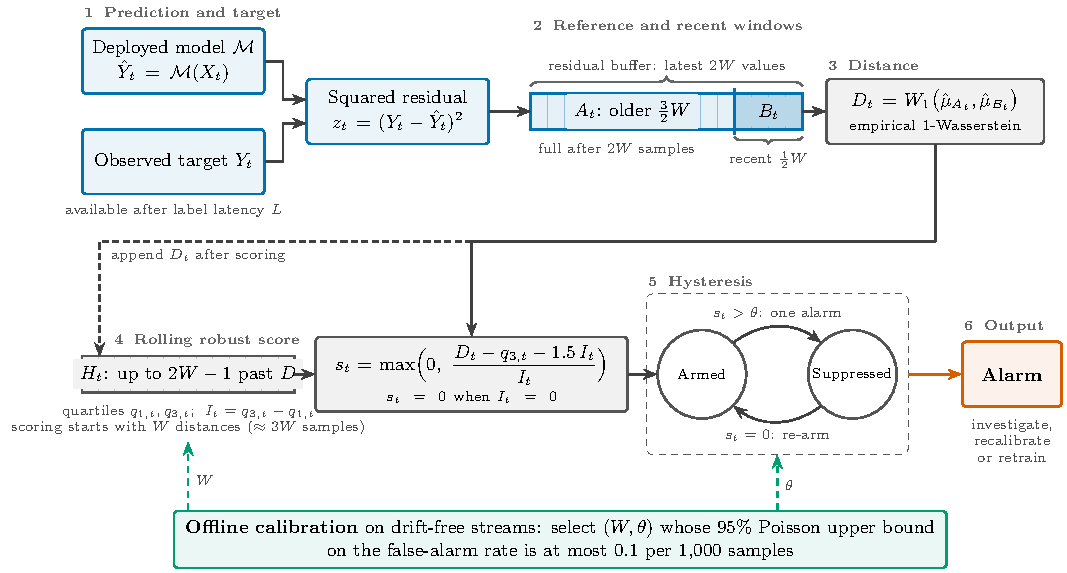
\includegraphics[width=\linewidth]{figures/pipeline.pdf}
\caption{End-to-end monitoring pipeline for per-sample testing ($B=1$). (1)~Each prediction is paired with its target once the target is observed, possibly after a label latency $L$. (2)~The latest $2W$ squared residuals are split into an older reference sample $A_t$ and a recent sample $B_t$. (3)~Their empirical $1$-Wasserstein distance $D_t$ is (4)~scored against the quartiles of up to $2W-1$ preceding distances. (5)~A two-state hysteresis emits one alarm when the score first exceeds $\theta$ and re-arms when the score returns to zero. (6)~The alarm can trigger investigation, recalibration or retraining. The window parameter $W$ and threshold $\theta$ are selected offline on drift-free streams under a common false-alarm budget (Section~\ref{sec:calibration}).}
\label{fig:pipeline}\end{figure}

\subsection{Monitored signal and distributional distance}
For a fixed deployed predictor $\mathcal M$ and observations $(X_t,Y_t)$, the detector monitors the squared error
\begin{equation}z_t=(Y_t-\mathcal M(X_t))^2.\end{equation}
An alarm says that two recent stretches of this stream look unusually different; it is a reason to investigate, not proof that the data-generating process has changed. Because squaring discards the sign, a change that flips the sign of errors while keeping their magnitude is invisible. The method could monitor any univariate signal, but every comparison here uses squared errors.

For distributions $\mu$ and $\nu$ on the real line with finite first moments, the $1$-Wasserstein distance is
\begin{equation}\label{eq:w1}
W_1(\mu,\nu)=\int_{\mathbb R}|F_\mu(x)-F_\nu(x)|\,dx.
\end{equation}
Because it integrates the gap between the two distribution functions over the whole line, it responds to differences anywhere in the distributions, including changes that leave the mean untouched.

Two further properties motivate the choice, and we cite them as background. $W_1$ is a metric on distributions with finite first moments~\cite{villani2008}, and in one dimension the empirical distance converges to the population distance at the rate $n^{-1/2}$ in the sample size $n$ under moment conditions~\cite{bobkov2019one}. Neither property distinguishes it from the Kolmogorov-Smirnov distance, which is also a metric between distribution functions and whose empirical version converges at the same rate.

The property that does distinguish them concerns changes that affect only part of the distribution. Suppose that a fraction $p$ of the probability mass changes, with $P=(1-p)R+pP_1$ before and $Q=(1-p)R+pQ_1$ after. Then $F_P-F_Q=p(F_{P_1}-F_{Q_1})$, so that
\begin{equation}\label{eq:mass}
\sup_x|F_P(x)-F_Q(x)|\leq p,\qquad W_1(P,Q)=p\,W_1(P_1,Q_1).
\end{equation}
The Kolmogorov-Smirnov distance cannot exceed the fraction of mass that moves, however far it moves, whereas the Wasserstein distance grows with the size of the displacement. The two are the $L^\infty$ and $L^1$ norms of $F_P-F_Q$. In one dimension the energy distance~\cite{szekely2013energy} equals $2\int_{\mathbb R}(F_P-F_Q)^2\,dx=2p^2\int_{\mathbb R}(F_{P_1}-F_{Q_1})^2\,dx$, a squared $L^2$ norm that also grows with the displacement but is quadratic in $p$. We therefore expect the Wasserstein distance to have an advantage when a change moves a small share of the errors far, and no particular advantage for changes in the shape of the bulk of the distribution. The same sensitivity to large displacements makes the distance on squared errors sensitive to outliers (Section~\ref{sec:limitations}).

\subsection{Windows and rolling score}
Let $W\geq2$ be an integer window parameter and let $t$ index residuals in arrival order. The detector keeps the latest $2W$ residuals and splits them into an older reference sample $A_t$ of size $\lfloor3W/2\rfloor$ and a recent sample $B_t$ holding the rest. Once the buffer is full, it computes $D_t=W_1(\hat\mu_{A_t},\hat\mu_{B_t})$ at every update. For even $W$ the windows are
\begin{equation}
A_t=(z_{t-2W+1},\ldots,z_{t-W/2}),\qquad
B_t=(z_{t-W/2+1},\ldots,z_t).
\end{equation}
The $3:1$ split gives the reference sample more observations; we fixed it in advance and did not tune it. Within one update the two samples do not overlap, but consecutive comparisons share most of their observations.

The distances go into a second buffer of up to $2W$ values. Scoring begins once it holds $W$ distances, which makes the initial warm-up roughly $3W$ samples long: the first score is available after $3W-1$ observations, and exposure calculations conservatively exclude the first $3W$. Let $H_t$ be the retained distances that precede $D_t$, excluding the current one; while scoring is active it contains between $W-1$ and $2W-1$ values. Its quartiles $q_{1,t}$ and $q_{3,t}$ are computed with NumPy's default linear percentile interpolation, and $I_t=q_{3,t}-q_{1,t}$. The score is
\begin{equation}\label{eq:score}
s_t=\begin{cases}
\displaystyle\frac{D_t-q_{3,t}-1.5I_t}{I_t},&I_t>0\text{ and }D_t>q_{3,t}+1.5I_t,\\
0,&\text{otherwise}.
\end{cases}
\end{equation}
A candidate alarm requires $s_t>\theta$ for a threshold $\theta\geq0$. When $I_t>0$ this is the same as $D_t>q_{3,t}+(1.5+\theta)I_t$, that is, Tukey's upper outlier fence~\cite{tukey1977exploratory} widened by $\theta I_t$. If the historical IQR is zero the score is set to zero, so a departure from a perfectly constant distance history is not scored until the history acquires some spread.

Quartiles limit the influence of extreme past distances on the scale estimate. The score is also scale invariant: multiplying every squared residual by a positive constant scales the distances, quartiles and IQR by the same factor, so in exact arithmetic neither the score nor the alarm sequence changes.
\subsection{Hysteresis and adaptation}
\label{sec:hysteresis}
The detector starts armed and then alternates between an armed and a suppressed state. While armed, a score above $\theta$ produces one alarm and moves the detector to the suppressed state. While suppressed, it stays silent and re-arms only when $s_t=0$, that is, when the current distance falls back inside the rolling fence or the IQR is zero. The re-arming rule is the same for every non-negative $\theta$.

Hysteresis never delays the first exceedance of an armed detector. It can, however, swallow the alarm for a second change if the excursion caused by the first has not yet ended. As monitoring continues, a persistent new regime fills both residual windows and then the distance history, so the reference updates itself without an explicit reset. By the same mechanism, a persistent change eventually becomes the new baseline whether or not it triggered an alarm, and a change that is slow enough may never be detected.

\subsection{Computational complexity and scope}
With sorting, the empirical distance costs $O(W\log W)$ time per update after warm-up, and the buffers need $O(W)$ memory. Throughout the study the predictor stays fixed after an alarm, and no retraining policy is evaluated. In operation, the suppressed state can be exposed alongside the alarm, so a persistent change remains visible without repeated alarms. If the predictor is retrained or replaced, the detector should be restarted with a fresh warm-up on residuals of the new model.

\section{Experimental Protocol}
\label{sec:validation}
\subsection{Streams, predictor and scenarios}
\label{sec:scenarios}
The main benchmark has seven synthetic scenarios grouped into five calibration families: linear abrupt, F1$\to$F2, F2$\to$F1, River Friedman and bimodal noise shift. The two directional function switches are evaluated on identical input and noise draws. Each monitoring stream has 20,000 samples, and the nominal change sits at zero-based index 15,000. For each family we generate 20 drift-free calibration streams and 50 test streams per scenario from separate seed ranges, plus 50 held-out null streams that we use to estimate placebo detection and null alarm rates. Within a comparison, all detectors see the same residual streams. The three River Friedman scenarios share calibration data and paired generator seeds, so they are not three independent families. Apart from the noise-level sweep of Section~\ref{sec:sensitivity}, every analysis in Sections~\ref{sec:results} and~\ref{sec:robustness} reuses each family's 50 test and 50 held-out null streams, so their results share the same evaluation-sample uncertainty.

An XGBoost regressor~\cite{chen2016} is fitted to 5,000 independently generated training observations, with 100 trees, maximum depth 5, learning rate 0.05, squared-error objective and random state 42. These hyperparameters were fixed in advance, with no early stopping or model selection. Each family uses one fitted predictor for its calibration, test and held-out null streams. Wasserstein and KSWIN receive raw squared errors. ADWIN and Page-Hinkley receive the squared errors divided by the median squared error of the family's pooled drift-free calibration streams, a constant fixed per family and fitted model, because ADWIN's bound assumes inputs in $[0,1]$ and Page-Hinkley's $\delta$ and threshold are expressed in units of the signal. Dividing by a positive constant leaves Wasserstein's alarms unchanged (Section~\ref{sec:method}), and KSWIN's Kolmogorov-Smirnov statistic depends only on the ordering of the observations; the real-world case of Section~\ref{sec:soil} applies the same division for every detector. No input is clipped, and no detector is reset at the known change point, so any alarm state from before the change carries into the detection horizon. \ref{app:generators} details the stream constructions, and \ref{app:parameters} lists the selected detector parameters.

The scenarios are:
\begin{enumerate}
\item \textbf{Linear abrupt:} a ten-dimensional linear relationship switches between two weight vectors, with uniform inputs and Gaussian noise of standard deviation 0.1.
\item \textbf{Friedman F1$\to$F2 and F2$\to$F1:} the input distribution stays fixed while the regression function switches between the first Friedman function~\cite{friedman1991multivariate} and a rescaled version of the second. The rescaling approximately matches the mean and standard deviation of the output, so what changes is the conditional relationship.
\item \textbf{River Friedman local and global abrupt:} the drifting Friedman generator of Ikonomovska et al.~\cite{ikonomovska2011learning}, as implemented in \texttt{river}. The local expanding abrupt (LEA) change replaces the regression function in two input regions, each defined by four of the inputs lying below 0.3 or above 0.7, and leaves it untouched elsewhere; with uniform inputs, the two regions hold a fraction $p=2\times0.3^4\approx0.016$ of the input mass. The global and slow gradual (GSG) change, used here with a transition window of zero, changes the regression function throughout the input space. Further generator change points fall outside the monitored interval.
\item \textbf{River Friedman transition window of 500 samples:} during the transition window the GSG generator picks the old or the new function with probability one half, and afterwards it uses only the new one. We do not report longer transition windows separately: with paired generator seeds they produce the same stream over the first 500 post-change samples, which is where most detections occur.
\item \textbf{Bimodal noise shift:} the linear regression function and input distribution remain fixed, while independent Gaussian noise $\varepsilon\sim\mathcal N(0,1)$ changes to
\begin{equation}\label{eq:mixture}
\varepsilon\sim\tfrac12\mathcal N(-\delta,1-\delta^2)+\tfrac12\mathcal N(\delta,1-\delta^2),\qquad0\leq\delta<1.
\end{equation}
The main benchmark uses $\delta=0.99$. The noise keeps mean zero and variance one; only its shape and higher moments change.
\end{enumerate}

We now derive which moments of the squared error the bimodal shift preserves. Write $a(X)=f(X)-\mathcal M(X)$ for the model's approximation error. Because the noise is independent with mean zero,
\begin{equation}\mathbb E[z\mid X]=a(X)^2+1\end{equation}
in both regimes, so the expected squared error is preserved even though the fitted model is imperfect. Its variance is not. By symmetry $\mathbb E[\varepsilon^3]=0$, and the noise in Eq.~\eqref{eq:mixture} has $\mathbb E[\varepsilon^4]=3-2\delta^4$, which gives
\begin{equation}
\operatorname{Var}(z\mid X)=4a(X)^2+2-2\delta^4,
\end{equation}
against $4a(X)^2+2$ under Gaussian noise. With the input distribution and predictor fixed, the unconditional variance of the squared error drops by $2\delta^4$. The change preserves the mean of the monitored loss but not its variance.

\subsection{Calibration under a false-alarm budget}
\label{sec:calibration}
Every candidate configuration is run on the 20 drift-free calibration streams. We call the exposure that remains after the protocol's initial warm-up exclusion ``active''; it still includes periods of hysteresis suppression and any recovery after later alarms. Calibration counts every alarm emitted on a stream but removes the conservative warm-up from the exposure denominator, so it can count an early scored alarm whose observations lie outside the denominator; for Wasserstein at batch size $B$ (Section~\ref{sec:batches}) the first score arrives after $3W-B$ observations. With $K$ recorded alarms over $E$ exposure samples, the pooled alarm rate is $1000K/E$, and the selection criterion is the one-sided 95\% Poisson upper bound
\begin{equation}\label{eq:ucb}
U=\frac{1000}{2E}\chi^2_{2(K+1),\,0.95}.
\end{equation}
Here $\chi^2_{\nu,p}$ denotes the $p$-quantile of a chi-squared distribution with $\nu$ degrees of freedom. The bound has its nominal coverage when the alarm count of a fixed configuration is Poisson. Overlapping windows, alarm suppression and the selection over many configurations all depart from that model, so we treat the bound as a selection rule and audit the chosen configurations on held-out null streams. A configuration is admissible when $U\leq0.1$. Among admissible configurations the procedure picks the highest observed rate, so as to come close to the budget, and breaks ties first by lower between-stream rate variability and then by a detector-specific parameter ordering. If no configuration is admissible, the one with the smallest upper bound is selected and reported as infeasible; this never happens in the main benchmark. Under a homogeneous Poisson working model, the budget corresponds to a probability of $1-\exp(-0.1)\approx0.095$ of at least one false alarm in a 1,000-sample horizon; the actual placebo probabilities are estimated empirically. In time units, $0.1$ alarms per 1,000 samples is about $0.9$ false alarms a year for hourly residuals and $8.6$ a day at one residual per second; the soil-moisture case of Section~\ref{sec:soil} keeps roughly the yearly rate for daily residuals, at $2.38$ per 1,000 days. In a deployment the budget should follow from the relative costs of a false alarm and a late detection; we use one value throughout for comparison, not as a recommendation.

Each calibration round gives the baselines 40 Optuna~\cite{akiba2019optuna} trials with a tree-structured Parzen estimator (TPE) sampler~\cite{bergstra2011algorithms}, ten startup trials and sampler seed 42. The initial search spaces are $\delta\in[10^{-5},0.1]$ for ADWIN; window size in $[500,1000]$, $\alpha\in[10^{-5},10^{-2}]$ and statistic size in $[20,80]$ for KSWIN; and threshold in $[50,500]$ and $\delta\in[10^{-5},5]$ for Page-Hinkley. Significance parameters and the Page-Hinkley $\delta$ are sampled on a logarithmic scale. ADWIN checks for a change at every sample, and KSWIN draws its random reference sample with seed 42. Besides its significance criterion, the River implementation of KSWIN requires an empirical KS statistic above 0.1; we leave this floor untuned. Page-Hinkley runs in two-sided mode with a forgetting factor of 0.9999 and a minimum of 30 observations before testing, all fixed.

For Wasserstein, the false-alarm constraint alone does not pin down the window, because every window in the sensitivity sweep admits some threshold that meets the budget (Section~\ref{sec:sensitivity}). We therefore choose the window by a fixed rule. The threshold, on the other hand, can be computed exactly. Hysteresis produces at most one alarm per positive-score excursion, where an excursion is a maximal run with $s_t>0$ that triggers if its maximum exceeds $\theta$. Over a full scored trajectory, the alarm count is thus the number of excursion maxima above $\theta$, and the lowest admissible threshold in $[0,64]$ follows directly from the calibration score trajectories. We try windows from 1,000 down to 500 in steps of 50 and keep the first that admits a threshold, together with that threshold. Every family ends up with $W=1000$: 24 alarms over 340,000 active samples, a rate of 0.071 and $U=0.099$. The reason why we prefer the longest window allowed is that longer windows accumulate more evidence against a persistent change. The rule and the search range were fixed before any test stream was evaluated. The upper end of 1,000 was set by the length of the streams, since the warm-up of about $3W$ samples and the exposure lost to it grow with $W$, and not by detection results. This treatment differs from that of the baselines, whose structural parameters, such as KSWIN's window, are searched together with their significance levels; for Wasserstein only the threshold is selected against the budget. Section~\ref{sec:sensitivity} reports detection at every window under the same budget.

A baseline's search range is widened when the selected configuration misses the budget, lies within 2\% of a search bound or produces no calibration alarms. The flagged end is extended by the current span (in log space for log-sampled parameters); a missed budget also extends the end that lowers the alarm rate, and a zero-alarm selection the end that raises it. After at most four extra rounds the selection rule is applied to the pooled trials. Widening looks only at calibration outcomes, but it gives the flagged detectors more trials. \ref{app:parameters} lists the selected parameters, widened ranges and trial counts.

The budget is a ceiling, and the selections approach it to different degrees. In the main benchmark every selected configuration raises between 23 and 29 calibration alarms, a rate of 0.058--0.073 per 1,000 active samples (Table~\ref{tab:params}). Only ADWIN needed a wider search, on F1$\to$F2, where its first selection lay at the lower end of the $\delta$ range; the final selection lies inside the widened range.

\subsection{Metrics and uncertainty}
\label{sec:metrics}
A stream counts as detected if an alarm falls in $[15000,16000)$. Over the detected streams we report the median first delay, with a 95\% percentile bootstrap interval from 2,000 resamples, and the mean and standard deviation. A delay of zero means an alarm on the first eligible post-change sample; missed streams are excluded from these summaries. We withhold conditional delays when fewer than five streams are detected, or when the lower Wilson bound for detection does not exceed the placebo point estimate, since such delays may come from chance alarms.

To bring misses into the speed comparison, we set $c_i=d_i$ for a detection with delay $0\leq d_i<H$ and $c_i=H$ otherwise, with $H=1000$. The mean horizon-capped delay $\bar c=n^{-1}\sum_i c_i$ appears next to the conditional delays (Table~\ref{tab:capped}). Lower values mean earlier or more frequent detection within the horizon, and the value depends on $H$ by construction.

For the main false-positive comparison we count pre-change alarms after the longest detector warm-up and divide by this shared exposure. Calibration and the Wasserstein-only studies instead use each detector's own active exposure, and the held-out null audit uses the full active exposure of the null streams. For Wasserstein at $W=1000$, the three exposures are 340,000 samples for calibration, 600,000 for the common pre-change comparison and 850,000 for the null audit.

Placebo detection is the fraction of held-out drift-free streams with an alarm in the same nominal horizon, and subtracting it from the detection rate gives excess detection. Flicker measures repeated alarms after the change: we count every alarm beyond the first over the whole 5,000-sample post-change interval and report the rate per 1,000 samples. Low flicker means something only alongside adequate detection, since a detector that rarely alarms also rarely repeats itself.

Delays are counted in residual samples from the change. In deployment the time from a change to an alarm is this delay converted to time at the observation cadence, plus the label latency $L$ (Figure~\ref{fig:pipeline}). The synthetic benchmark assumes that every target is observed, in order; missing or irregularly delayed targets are not modelled.

Detection and placebo proportions come with 95\% Wilson score intervals~\cite{wilson1927probable}, which stay informative at proportions of 0 and 1; Table~\ref{tab:wilson} gives them for every proportion in the main results. Delay intervals resample streams, and null-rate intervals resample whole null streams, which preserves the dependence between alarms on the same stream. All intervals are conditional on the fitted model and the selected detector parameters.

\subsection{Statistical comparisons}
\label{sec:significance}
Paired Wilcoxon signed-rank tests~\cite{wilcoxon1945individual} compare first delays on jointly detected streams and false-alarm counts on the common pre-change interval, and exact McNemar tests~\cite{mcnemar1947note} compare paired detected/missed outcomes. All tests are two-sided at a family-wise level of 0.05. Holm correction~\cite{holm1979simple} is applied separately to the delay and the detection families, each covering all 21 scenario--baseline comparisons. The three River Friedman scenarios share their pre-change streams and hence their false-alarm counts, so these are tested once, leaving 15 comparisons in the false-alarm family. Because delay tests condition on both methods detecting, detection power is compared separately through the McNemar tests.

As a complementary analysis, we run Friedman tests with Nemenyi post-hoc comparisons~\cite{demvsar2006statistical} within each scenario, using streams as blocks and giving missed detections the worst delay rank. The omnibus tests are Holm-corrected across scenarios, and Nemenyi comparisons use $\alpha=0.05/7$. The batch-size analyses repeat these correction families within each batch size, with no joint correction across batch sizes and no inferential comparison between them.

\section{Main Results}
\label{sec:results}
\subsection{Coverage across abrupt change scenarios}
\label{sec:coverage}
The Wasserstein detector stays well above placebo in every one of the seven scenarios (Figure~\ref{fig:main} and Table~\ref{tab:main}). It detects 48 to 50 of the 50 streams in every scenario, with excess detection between 0.90 and 0.94. Each baseline, in contrast, has at least one scenario in which it detects drift no more often than it alarms on null streams: the minimum excess detection is $-0.04$ for KSWIN and ADWIN and $-0.08$ for Page-Hinkley. Excess detection is a difference of two point estimates; Table~\ref{tab:wilson} gives the Wilson intervals of both. In five scenarios every detector finds at least 94\% of the changes, so the contrast in coverage comes from two scenarios, local abrupt drift and bimodal shift, and holds for this suite of abrupt single changes. Within individual scenarios the leading detectors differ by at most 0.06 in excess detection, within the sampling uncertainty of Table~\ref{tab:wilson}: Wasserstein ties with ADWIN for the highest value on local abrupt, global abrupt and transition drift, ADWIN and Page-Hinkley lead slightly on linear abrupt drift, and KSWIN on F1$\to$F2, F2$\to$F1 and bimodal shift. The advantage of the Wasserstein detector is therefore consistency across change types, not superiority in any single one.

\begin{figure}[htbp]\centering
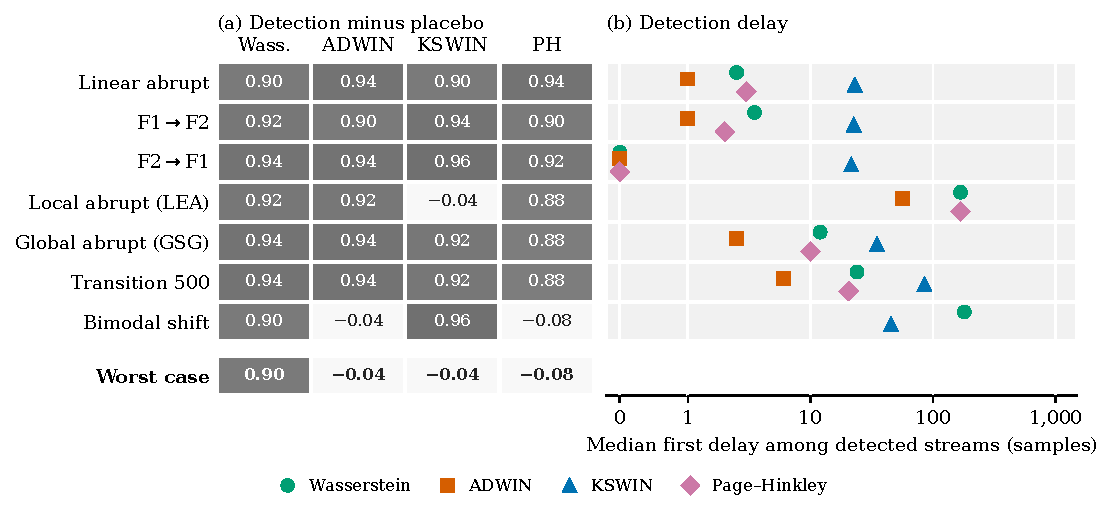
\includegraphics[width=\linewidth]{figures/main_coverage_delay.pdf}
\caption{Main benchmark summary. (a)~Detection rate minus held-out placebo rate per scenario, with the minimum over scenarios in the bottom row; darker cells denote larger excess detection, and negative values are shaded as zero. (b)~Median first delay among detected streams, on a logarithmic scale that is linear below one sample. No marker is drawn where the conditional-delay reporting criterion fails: KSWIN on local abrupt drift (2 of 50) and ADWIN and Page-Hinkley on bimodal shift (1 of 50 each). Values are those of Table~\ref{tab:main}.}
\label{fig:main}\end{figure}

The baselines fail on different changes. KSWIN detects only two of the 50 local-drift streams, against 48 for Wasserstein, with a placebo rate of 0.08. On bimodal shift, ADWIN and Page-Hinkley detect one stream each, against 49 for Wasserstein, with placebo rates of 0.06 and 0.10. These three contrasts are the only significant ones in the Holm-corrected McNemar analysis (Table~\ref{tab:mcnemar}), and none of the configurations involved had its search range widened.

These failures follow largely from what each statistic measures. ADWIN and Page-Hinkley track mean-related quantities, and the bimodal construction preserves the expected squared error (Section~\ref{sec:scenarios}). KSWIN's difficulty with local drift has a different origin, the mass bound of Eq.~\eqref{eq:mass}. The LEA change alters the regression function only on inputs that hold a fraction $p\approx0.016$ of the input mass (Section~\ref{sec:scenarios}), so the residual distribution is a mixture of the kind assumed there, and the population KS distance between pre- and post-change squared residuals cannot exceed about 0.016, however large the new errors in the affected regions are. The Wasserstein distance, by contrast, grows with the size of those errors. KSWIN's fixed floor of 0.1 on the empirical statistic plays no role: at every selected significance level and statistic sample size, significance already requires an empirical KS statistic of at least 0.375 in the main benchmark, and 0.27 at every batch size. Larger statistic samples would lower this requirement, but not enough to matter here: at the significance levels selected for the River Friedman family, a population KS distance of 0.016 reaches the asymptotic two-sample critical value only with about 39,000 observations in each sample in the main benchmark and at least 20,000 at every batch size, far more than the 1,000-sample detection horizon provides. The ablation points the same way: the KS statistic inside our detector also loses local-drift detection at the same budget (Section~\ref{sec:ablation}). The KS statistic is far from blind to shape changes, however: on bimodal shift KSWIN detects all 50 streams, including the one Wasserstein misses.

This blind spot of ADWIN and Page-Hinkley is not peculiar to squared residuals. For any transform $g$ of the residual, a detector that tracks the mean of $g(e)$ cannot respond to a change that preserves $\mathbb E[g(e)]$. A distributional detector applied to the same signal misses only changes that preserve the whole law of $g(e)$, a subset of the former. Changing the monitored signal moves the blind spot of a mean-based detector but does not remove it, and the same holds for a detector that tracks any finite set of moments of $g(e)$, such as a mean and a variance. We therefore keep squared residuals, the quantity the fitted predictor minimises, as the common signal, and regard the bimodal scenario as one member of a class of changes that every mean-based detector admits. The specific failures reported here hold for squared residuals: ADWIN and Page-Hinkley reading absolute residuals could respond to this bimodal change, which raises the mean absolute error, but would be blind to a different mixture change; we did not evaluate such variants.

\begingroup\small\setlength{\tabcolsep}{4pt}
\begin{longtable}{lrrrrrr}
\caption{Main benchmark, 50 test streams per scenario. Det. is detection within 1,000 samples; Pl. is detection in the corresponding horizon on held-out null streams. Delays are in samples among detected streams: median with a 95\% bootstrap interval, and mean $\pm$ standard deviation; n/a marks outcomes failing the conditional-delay reporting criterion (fewer than five, or a Wilson lower bound not above the placebo rate). FP uses the common pre-drift exposure. FP and flicker are alarms per 1,000 samples.}\label{tab:main}\\
\toprule
Detector & Det. & Pl. & Median delay & Mean delay & FP & Flicker\\\midrule\endfirsthead
\multicolumn{7}{l}{\small Table \thetable\ continued}\\\toprule
Detector & Det. & Pl. & Median delay & Mean delay & FP & Flicker\\\midrule\endhead
\bottomrule\endfoot
\multicolumn{7}{l}{\textit{Linear abrupt}}\\*
Wasserstein & 1.00 & 0.10 & 2.5 [2.0, 3.0] & $3.0 \pm 2.2$ & 0.073 & 0.03\\*
ADWIN & 0.98 & 0.04 & 1.0 [0.0, 1.0] & $1.1 \pm 1.3$ & 0.073 & 0.06\\*
KSWIN & 0.94 & 0.04 & 23.0 [22.0, 24.0] & $31.6 \pm 41.5$ & 0.092 & 0.08\\*
Page-Hinkley & 1.00 & 0.06 & 3.0 [2.5, 5.0] & $3.9 \pm 2.7$ & 0.067 & 30.80\\
\addlinespace
\multicolumn{7}{l}{\textit{F1$\to$F2}}\\*
Wasserstein & 1.00 & 0.08 & 3.5 [2.0, 4.0] & $4.1 \pm 3.4$ & 0.063 & 0.02\\*
ADWIN & 0.98 & 0.08 & 1.0 [1.0, 2.0] & $1.3 \pm 1.3$ & 0.057 & 0.00\\*
KSWIN & 1.00 & 0.06 & 22.5 [21.0, 24.0] & $34.1 \pm 59.2$ & 0.072 & 0.04\\*
Page-Hinkley & 1.00 & 0.10 & 2.0 [2.0, 4.0] & $3.0 \pm 1.9$ & 0.053 & 32.87\\
\addlinespace
\multicolumn{7}{l}{\textit{F2$\to$F1}}\\*
Wasserstein & 1.00 & 0.06 & 0.0 [0.0, 0.0] & $0.3 \pm 0.5$ & 0.058 & 0.02\\*
ADWIN & 0.98 & 0.04 & 0.0 [0.0, 0.0] & $0.2 \pm 0.4$ & 0.067 & 0.04\\*
KSWIN & 1.00 & 0.04 & 21.5 [20.5, 22.0] & $23.3 \pm 18.8$ & 0.065 & 0.06\\*
Page-Hinkley & 1.00 & 0.08 & 0.0 [0.0, 0.0] & $0.7 \pm 2.5$ & 0.068 & 33.20\\
\addlinespace
\multicolumn{7}{l}{\textit{Local abrupt (LEA)}}\\*
Wasserstein & 0.96 & 0.04 & 167.5 [131.5, 241.6] & $203.7 \pm 144.9$ & 0.065 & 0.03\\*
ADWIN & 0.98 & 0.06 & 56.0 [40.0, 142.0] & $114.4 \pm 108.6$ & 0.092 & 0.41\\*
KSWIN & 0.04 & 0.08 & n/a & n/a & 0.032 & 0.00\\*
Page-Hinkley & 1.00 & 0.12 & 167.5 [142.5, 253.0] & $200.0 \pm 135.1$ & 0.085 & 2.22\\
\addlinespace
\multicolumn{7}{l}{\textit{Global abrupt (GSG)}}\\*
Wasserstein & 0.98 & 0.04 & 12.0 [10.0, 15.0] & $12.9 \pm 7.4$ & 0.065 & 0.02\\*
ADWIN & 1.00 & 0.06 & 2.5 [1.0, 4.5] & $3.2 \pm 2.6$ & 0.092 & 0.04\\*
KSWIN & 1.00 & 0.08 & 35.0 [31.0, 37.0] & $33.6 \pm 8.0$ & 0.032 & 0.05\\*
Page-Hinkley & 1.00 & 0.12 & 10.0 [7.5, 12.0] & $11.5 \pm 7.8$ & 0.085 & 11.90\\
\addlinespace
\multicolumn{7}{l}{\textit{Transition 500}}\\*
Wasserstein & 0.98 & 0.04 & 24.0 [19.0, 31.0] & $26.8 \pm 16.2$ & 0.065 & 0.02\\*
ADWIN & 1.00 & 0.06 & 6.0 [4.5, 8.0] & $8.0 \pm 8.0$ & 0.092 & 0.26\\*
KSWIN & 1.00 & 0.08 & 85.0 [68.0, 131.5] & $198.1 \pm 207.6$ & 0.032 & 0.15\\*
Page-Hinkley & 1.00 & 0.12 & 20.5 [17.0, 27.5] & $23.1 \pm 15.0$ & 0.085 & 11.43\\
\addlinespace
\multicolumn{7}{l}{\textit{Bimodal shift}}\\*
Wasserstein & 0.98 & 0.08 & 180.0 [168.0, 212.0] & $200.0 \pm 71.1$ & 0.037 & 0.02\\*
ADWIN & 0.02 & 0.06 & n/a & n/a & 0.060 & 0.00\\*
KSWIN & 1.00 & 0.04 & 45.5 [42.0, 48.0] & $44.3 \pm 8.4$ & 0.053 & 0.02\\*
Page-Hinkley & 0.02 & 0.10 & n/a & n/a & 0.070 & 0.00\\
\addlinespace
\end{longtable}\endgroup

\subsection{Detection speed and alarm behaviour}
\label{sec:speed}
ADWIN is usually the fastest detector (Figure~\ref{fig:main}b). Its conditional delays are significantly shorter than Wasserstein's on every functional change except F2$\to$F1, most clearly on local abrupt drift, with a median of 56.0 against 167.5 samples. KSWIN is significantly slower than Wasserstein on five functional-change scenarios but significantly faster on bimodal shift, with a median of 45.5 against 180.0 samples. On the five Friedman-based scenarios, Page-Hinkley's delays do not differ significantly from Wasserstein's.

On F2$\to$F1, Wasserstein and ADWIN do not differ significantly, and both have a median delay of zero. On linear abrupt drift Wasserstein is significantly faster than KSWIN and than Page-Hinkley; in the latter contrast the median paired difference is zero, but Page-Hinkley is slower on 23 of the 28 jointly detected streams whose delays differ. No pairwise false-positive contrast survives correction. Wasserstein's pre-change rates of 0.037--0.073 per 1,000 common-exposure samples stay below the budget, as do its held-out null rates of 0.060--0.076 per 1,000 active samples, and every detector's held-out rate lies below its calibration upper bound.

Repeated alarms after the change separate the detectors more sharply. Wasserstein's flicker is 0.02--0.03 per 1,000 post-change samples, KSWIN's 0.00--0.15 and ADWIN's 0.00--0.41, whereas Page-Hinkley reaches 11.43--33.20 on four of the five Friedman-based scenarios and 30.80 on linear abrupt drift. These numbers reflect how each detector manages its alarm state as much as what it detects: in the implementations compared here, Page-Hinkley and ADWIN reset their state after an alarm and can alarm again while a change persists, KSWIN must refill its window before testing again, and Wasserstein suppresses repeats until its score returns to zero. The ablation in Section~\ref{sec:ablation} shows that hysteresis is what keeps repeats low in our detector.

The per-scenario Friedman rankings (\ref{app:statistics}) agree: ADWIN has the best average delay rank on all six functional-change scenarios and KSWIN on bimodal shift, although ADWIN's lead over Wasserstein stays inside the Nemenyi critical difference on F2$\to$F1 and linear abrupt drift.


\begin{table}[htbp]\centering\small
\caption{Mean horizon-capped delay over all 50 streams, in samples. Misses receive the 1,000-sample cap.}\label{tab:capped}
\setlength{\tabcolsep}{5pt}\begin{tabular}{lrrrr}
\toprule
Scenario & Wasserstein & ADWIN & KSWIN & PH\\\midrule
Linear abrupt & 2.98 & 21.06 & 89.70 & 3.86\\
F1$\to$F2 & 4.14 & 21.32 & 34.10 & 3.04\\
F2$\to$F1 & 0.30 & 20.20 & 23.28 & 0.68\\
Local abrupt (LEA) & 235.56 & 132.10 & 980.18 & 199.98\\
Global abrupt (GSG) & 32.62 & 3.16 & 33.62 & 11.50\\
Transition 500 & 46.24 & 8.04 & 198.12 & 23.14\\
Bimodal shift & 216.02 & 997.26 & 44.28 & 987.44\\
\bottomrule
\end{tabular}\end{table}

Counting misses changes some of these comparisons (Table~\ref{tab:capped}). ADWIN is faster on linear abrupt and F1$\to$F2 when it detects, but a single miss in each of these scenarios and in F2$\to$F1 raises its capped mean delay to 20.20--21.32 samples, against 0.30--4.14 for Wasserstein. Page-Hinkley has the lowest capped mean on F1$\to$F2, ADWIN on the three River scenarios and KSWIN on bimodal shift, where ADWIN and Page-Hinkley sit close to the 1,000-sample cap.

\section{Diagnostic Experiments}
\label{sec:robustness}
\subsection{Mixture-separation sweep}
\label{sec:severity}
To measure how strong a shape change must be before it is detected, we vary only $\delta$ in Eq.~\eqref{eq:mixture}, keeping each detector's calibrated parameters, which remain valid because separation affects only the post-change noise. Every level uses the same 50 generator seeds and input streams.

\begin{table}[htbp]\centering\small
\caption{Mixture-separation sweep with fixed calibrated parameters and the same 50 test streams at every level. Separation affects only the post-change noise. The held-out placebo rates are 0.06, 0.04, 0.10 and 0.08 for ADWIN, KSWIN, Page-Hinkley and Wasserstein, respectively.}\label{tab:severity}
\setlength{\tabcolsep}{4pt}\begin{tabular}{rrrrr}
\toprule
$\delta$ & ADWIN & KSWIN & Page-Hinkley & Wasserstein\\\midrule
0.25 & 0.06 & 0.04 & 0.12 & 0.00\\
0.40 & 0.04 & 0.06 & 0.08 & 0.00\\
0.55 & 0.02 & 0.02 & 0.08 & 0.00\\
0.70 & 0.00 & 0.04 & 0.08 & 0.00\\
0.85 & 0.00 & 0.38 & 0.06 & 0.34\\
0.95 & 0.00 & 1.00 & 0.04 & 0.92\\
0.99 & 0.02 & 1.00 & 0.02 & 0.98\\
\bottomrule\end{tabular}\end{table}

Wasserstein detects 0.98 of the streams at $\delta=0.99$, 0.92 at 0.95 and 0.34 at 0.85, and none from 0.70 down to 0.25; with four placebo alarms in 50 null streams, these zeros give no evidence of detection at the weaker settings. KSWIN detects every stream at 0.95 and 0.38 at 0.85 before it too drops to placebo level. ADWIN and Page-Hinkley stay near or below their placebo rates throughout, consistent with their low sensitivity to a change that preserves the mean.

For $\delta\leq1/\sqrt2$ the symmetric mixture is not bimodal, although it still differs from the Gaussian reference; both distributional detectors respond once the noise becomes clearly bimodal, while the mean-based detectors stay at placebo level even at the strongest separation. KSWIN's observed detection rate is at least as high as Wasserstein's at every separation, and the two are close at 0.85.

\begin{figure}[htbp]\centering
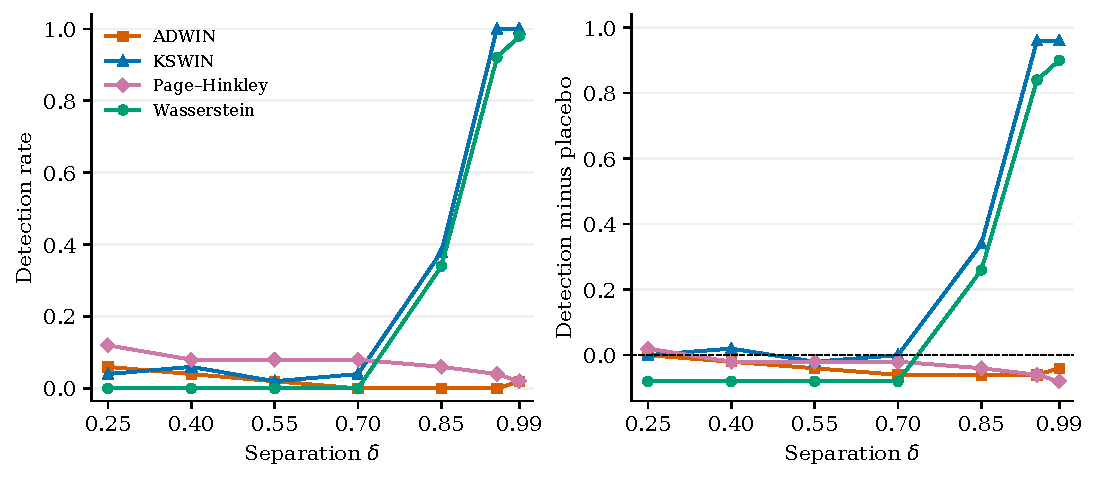
\includegraphics[width=\linewidth]{figures/severity_current.pdf}
\caption{Detection and excess detection across the mixture-separation sweep. Lines connect evaluated settings only. Parameters remain fixed across the sweep; the horizontal zero line in the right panel denotes detection equal to the held-out placebo rate.}
\label{fig:severity}\end{figure}

\subsection{Repeated calibration}
\label{sec:calibration-robustness}
To check how much the results depend on the particular calibration streams, we repeat the Wasserstein calibration five times on linear abrupt, local abrupt and bimodal shift, each time with a disjoint range of calibration seeds, while keeping each family's fitted model, test residuals and null residuals fixed. None of the repetitions reuses the main benchmark's calibration data.

\begin{table}[htbp]\centering\small
\caption{Calibration repetitions for Wasserstein. Each repetition uses different calibration streams; the fitted model, 50 test streams and held-out null streams remain fixed within a family. Every repetition selects $W=1000$. Delays are among detected streams. Null FP is the alarm rate per 1,000 active samples on the held-out null streams. All 15 configurations pass the calibration UCB criterion. $^\ast$~Held-out rate above the budget.}\label{tab:robust}
\setlength{\tabcolsep}{4pt}\begin{tabular}{rrrrrrr}
\toprule
Rep. & $\theta$ & Det. & Median & Mean & Null FP & Pl.\\\midrule
\multicolumn{7}{l}{\textit{Linear abrupt}}\\*
1 & 2.027 & 1.00 & 3.0 & 3.1 & 0.048 & 0.08\\*
2 & 1.782 & 1.00 & 2.5 & 3.0 & 0.066 & 0.10\\*
3 & 1.999 & 1.00 & 3.0 & 3.1 & 0.049 & 0.08\\*
4 & 1.719 & 1.00 & 2.5 & 2.9 & 0.071 & 0.12\\*
5 & 2.094 & 1.00 & 3.0 & 3.1 & 0.040 & 0.08\\
\addlinespace
\multicolumn{7}{l}{\textit{River Friedman (LEA)}}\\*
1 & 1.946 & 0.96 & 167.5 & 203.4 & 0.060 & 0.04\\*
2 & 1.887 & 0.96 & 167.5 & 202.5 & 0.061 & 0.06\\*
3 & 1.714 & 0.96 & 154.0 & 195.3 & 0.080 & 0.06\\*
4 & 1.719 & 0.96 & 157.5 & 196.6 & 0.079 & 0.06\\*
5 & 1.702 & 0.96 & 154.0 & 193.5 & 0.080 & 0.06\\
\addlinespace
\multicolumn{7}{l}{\textit{Bimodal shift}}\\*
1 & 1.736 & 1.00 & 174.5 & 194.9 & 0.082 & 0.08\\*
2 & 1.546 & 1.00 & 169.0 & 184.4 & 0.105$^\ast$ & 0.12\\*
3 & 1.797 & 1.00 & 178.5 & 202.2 & 0.079 & 0.08\\*
4 & 1.676 & 1.00 & 172.0 & 192.1 & 0.088 & 0.10\\*
5 & 1.906 & 0.98 & 180.0 & 200.8 & 0.067 & 0.06\\
\addlinespace
\bottomrule\end{tabular}\end{table}

Every repetition again selects $W=1000$, with thresholds between 1.55 and 2.09, and detection on these evaluation streams barely moves across the five calibration draws (Table~\ref{tab:robust}). The held-out null rates vary more, from 0.040 to 0.105 alarms per 1,000 active samples; one bimodal repetition lies slightly above the budget, with a 95\% whole-stream bootstrap interval of $[0.0894,0.1200]$ that contains 0.1.

\subsection{Ablations at a matched false-alarm budget}
\label{sec:ablation}
The ablation compares the full detector with four variants: no hysteresis, a mean/standard-deviation bound, a KS statistic~\cite{massey1951kolmogorov} and an energy-distance statistic~\cite{szekely2013energy}. The mean/SD variant uses $\mu+1.5\sigma$ as its baseline fence and divides the excess by $\sigma$, keeping everything else. The KS and energy variants keep the original windows, IQR score and hysteresis, so the KS variant differs from the KSWIN baseline. Each variant goes through the main benchmark's calibration, window rule included; all select $W=1000$ and raise the same 24 calibration alarms (0.071 per 1,000 samples), and the full variant reproduces the main Wasserstein results (\ref{app:ablation}).

The full detector has the highest minimum excess detection, 0.90. Without hysteresis the minimum drops to 0.74, and with the mean/SD bound in place of the IQR bound to 0.68, both on bimodal shift. Replacing the statistic gives minima of $-0.02$ for KS and 0.32 for energy distance, both on local drift. At its recalibrated operating point, then, each component contributes, and each matters for a different type of change.

Without hysteresis every step above the threshold is a separate alarm, so meeting the budget takes thresholds of 4.19--6.08 instead of 1.73--1.95. The higher threshold costs both power and speed: bimodal detection falls from 0.98 to 0.74 and local detection from 0.96 to 0.88, median delays grow in every scenario except F2$\to$F1, and repeated post-change alarms rise to 39.6--114.3 per 1,000 samples. The placebo rate, on the other hand, is zero in every scenario, plausibly because counting every exceedance packs the fixed number of calibration alarms into fewer excursions; zero detected null horizons out of 50 still leave a Wilson upper limit of about 0.071.

The mean/SD bound detects 37 of the 50 bimodal streams, against 49 with the IQR bound. On the functional changes it detects as often as the full detector, apart from one stream on F1$\to$F2, and slightly sooner, but its placebo rate on the River Friedman scenarios is 0.10 instead of 0.04.

Swapping the statistic matters most for local drift, where detection is 0.96 with Wasserstein, 0.04 with KS and 0.34 with energy distance, all at matched calibration alarm rates. The ordering follows Eq.~\eqref{eq:mass}: the KS statistic is capped by the small affected mass, the energy distance grows with the displacement but is quadratic in that mass, and the Wasserstein distance is linear in it. The substitutes are also slower on the functional changes. Bimodal shift reverses the order: both detect all 50 streams, with median delays of 102.5 for KS and 142.0 for energy distance against 180.0 for Wasserstein, in line with KSWIN's advantage in the main benchmark.

\subsection{Hyperparameter and noise sensitivity}
\label{sec:sensitivity}
We next look at the neighbourhood of each family's calibrated setting $(W^*,\theta^*)$, where $W^*=1000$ throughout. For each $W\in\{500,600,750,900,1000\}$ we compute the lowest threshold that meets the budget; a separate threshold sweep holds $W^*$ fixed, and on linear abrupt drift we also vary the noise level, recalibrating the threshold at each level. \ref{app:sensitivity} reports all settings.

At a matched budget, the window mainly trades sensitivity to the bimodal change against delay. Bimodal detection rises steadily with the window, from 0.82 at $W=500$ to 0.98 at $W=1000$, while the conditional median delay stays between 166.0 and 180.0 samples; because fewer streams are missed, the mean horizon-capped delay improves from 315.8 to 216.0 samples. On the functional changes detection stays at 0.96--1.00, and smaller windows react slightly sooner: on local drift the median delay is 135.0 samples at $W=500$ against 167.5 at $W=1000$. When functional changes like these are the main concern and short conditional delays matter most, smaller windows are worth considering.

The threshold traces the trade-off between delay and false alarms, with $\theta^*$ sitting at the edge of the budget by construction. On linear abrupt drift, $\theta=1.5$ already breaks the budget, and at $\theta=0$ placebo detection rises to 0.48 and calibration alarms to 1.93 per 1,000 samples, against 0.10 and 0.071 at $\theta^*=1.78$, while the median delay falls only from 2.5 to 2.0 samples. Raising $\theta$ to 4 lowers detection to 0.90 on local drift and 0.84 on bimodal shift. Lowering the threshold can also cost detection. At $\theta=0$ detection falls to 0.96 on F1$\to$F2 and 0.94 on F2$\to$F1, whereas at $\theta=4$ the single stream that the calibrated detector misses on global abrupt and transition drift is detected. Both effects are what one would expect if a pre-change alarm opened an excursion that had not ended when the change arrived, so that hysteresis suppressed the post-change alarm (Section~\ref{sec:hysteresis}). Raising the noise standard deviation on linear abrupt drift from 0.05 to 0.4 keeps detection at 1.00 within the budget, while the median delay grows from 2.0 to 18.0 samples.

\subsection{Residuals arriving in batches}
\label{sec:batches}
In deployment, targets often arrive in blocks, for instance once a day, and a detector may only be consulted when a block is complete. We therefore repeat the main benchmark with residuals delivered in batches of $B\in\{10,50,100\}$ samples. Every detector still reads every residual but can alarm only on the last sample of a batch. Wasserstein computes its distance once per batch and keeps up to $2\lceil W/B\rceil$ distances, so its history spans roughly the same stretch of the stream as without batching but contains fewer distances: at $W=1000$ and $B=100$ the buffer holds at most 20 distances and the fence uses at most 19 preceding ones, compared with 1,999 at $B=1$. Batching thus changes the adaptive score as well as the opportunities to alarm. ADWIN, KSWIN and Page-Hinkley update their state with every residual but test only at the end of a batch. Because a different testing frequency may admit a more sensitive setting, each batch size is calibrated separately under the protocol of Section~\ref{sec:calibration}, with the same streams, budget and horizon. Delays are still counted in samples; the change at index 15,000 starts a batch for every $B$, so the shortest possible delay is $B-1$. Table~\ref{tab:batch} reports all batch sizes, including the main benchmark at $B=1$.

\begingroup\small\setlength{\tabcolsep}{4pt}
\begin{longtable}{rrrrrrrrr}
\caption{Detection and conditional median delay for all evaluated batch sizes, with separate calibration at each size. Det. is detection within 1,000 samples. Delays include the wait for the batch boundary; the shortest possible delay is $B-1$. Entries marked n/a fail the conditional-delay reporting criterion. $B=1$ reproduces Table~\ref{tab:main}. PH denotes Page-Hinkley.}\label{tab:batch}\\
\toprule
& \multicolumn{4}{c}{Det.} & \multicolumn{4}{c}{Median delay}\\\cmidrule(lr){2-5}\cmidrule(lr){6-9}
$B$ & Wass. & ADWIN & KSWIN & PH & Wass. & ADWIN & KSWIN & PH\\\midrule\endfirsthead
\multicolumn{9}{l}{\small Table \thetable\ continued}\\
\toprule
& \multicolumn{4}{c}{Det.} & \multicolumn{4}{c}{Median delay}\\\cmidrule(lr){2-5}\cmidrule(lr){6-9}
$B$ & Wass. & ADWIN & KSWIN & PH & Wass. & ADWIN & KSWIN & PH\\\midrule\endhead
\bottomrule\endfoot
\multicolumn{9}{l}{\textit{Linear abrupt}}\\*
1 & 1.00 & 0.98 & 0.94 & 1.00 & 2.5 & 1.0 & 23.0 & 3.0\\*
10 & 1.00 & 0.98 & 0.98 & 1.00 & 9.0 & 9.0 & 29.0 & 9.0\\*
50 & 1.00 & 0.98 & 0.98 & 1.00 & 49.0 & 49.0 & 49.0 & 49.0\\*
100 & 1.00 & 0.98 & 1.00 & 1.00 & 99.0 & 99.0 & 99.0 & 99.0\\
\addlinespace
\multicolumn{9}{l}{\textit{F1$\to$F2}}\\*
1 & 1.00 & 0.98 & 1.00 & 1.00 & 3.5 & 1.0 & 22.5 & 2.0\\*
10 & 1.00 & 0.98 & 0.98 & 1.00 & 9.0 & 9.0 & 29.0 & 9.0\\*
50 & 1.00 & 0.96 & 1.00 & 1.00 & 49.0 & 49.0 & 49.0 & 49.0\\*
100 & 0.98 & 0.96 & 1.00 & 1.00 & 99.0 & 99.0 & 99.0 & 99.0\\
\addlinespace
\multicolumn{9}{l}{\textit{F2$\to$F1}}\\*
1 & 1.00 & 0.98 & 1.00 & 1.00 & 0.0 & 0.0 & 21.5 & 0.0\\*
10 & 1.00 & 0.98 & 0.98 & 1.00 & 9.0 & 9.0 & 19.0 & 9.0\\*
50 & 1.00 & 0.98 & 0.98 & 1.00 & 49.0 & 49.0 & 49.0 & 49.0\\*
100 & 0.98 & 0.98 & 0.98 & 1.00 & 99.0 & 99.0 & 99.0 & 99.0\\
\addlinespace
\multicolumn{9}{l}{\textit{Local abrupt (LEA)}}\\*
1 & 0.96 & 0.98 & 0.04 & 1.00 & 167.5 & 56.0 & n/a & 167.5\\*
10 & 0.96 & 0.98 & 0.00 & 1.00 & 174.0 & 59.0 & n/a & 59.0\\*
50 & 0.96 & 0.98 & 0.12 & 1.00 & 174.0 & 99.0 & n/a & 199.0\\*
100 & 0.96 & 0.98 & 0.04 & 1.00 & 199.0 & 199.0 & n/a & 199.0\\
\addlinespace
\multicolumn{9}{l}{\textit{Global abrupt (GSG)}}\\*
1 & 0.98 & 1.00 & 1.00 & 1.00 & 12.0 & 2.5 & 35.0 & 10.0\\*
10 & 0.98 & 1.00 & 1.00 & 1.00 & 19.0 & 9.0 & 34.0 & 9.0\\*
50 & 0.98 & 0.98 & 0.86 & 1.00 & 49.0 & 49.0 & 49.0 & 49.0\\*
100 & 0.98 & 0.98 & 0.98 & 1.00 & 99.0 & 99.0 & 99.0 & 99.0\\
\addlinespace
\multicolumn{9}{l}{\textit{Transition 500}}\\*
1 & 0.98 & 1.00 & 1.00 & 1.00 & 24.0 & 6.0 & 85.0 & 20.5\\*
10 & 0.98 & 1.00 & 0.98 & 1.00 & 29.0 & 9.0 & 119.0 & 9.0\\*
50 & 0.98 & 1.00 & 0.32 & 1.00 & 49.0 & 49.0 & 549.0 & 49.0\\*
100 & 0.98 & 1.00 & 0.88 & 1.00 & 99.0 & 99.0 & 99.0 & 99.0\\
\addlinespace
\multicolumn{9}{l}{\textit{Bimodal shift}}\\*
1 & 0.98 & 0.02 & 1.00 & 0.02 & 180.0 & n/a & 45.5 & n/a\\*
10 & 1.00 & 0.02 & 0.96 & 0.00 & 179.0 & n/a & 39.0 & n/a\\*
50 & 1.00 & 0.00 & 0.96 & 0.02 & 199.0 & n/a & 49.0 & n/a\\*
100 & 1.00 & 0.00 & 0.96 & 0.00 & 199.0 & n/a & 99.0 & n/a\\
\addlinespace
\end{longtable}\endgroup

Batching leaves the coverage pattern of Section~\ref{sec:coverage} intact. Wasserstein detects 0.96--1.00 of the streams in every scenario at every batch size, while ADWIN and Page-Hinkley detect at most one bimodal stream and KSWIN at most six local-drift streams; the corresponding McNemar contrasts with Wasserstein remain significant after Holm correction throughout.

Batching compresses the differences in speed. At $B=100$ every detector has a median delay of 99 samples on linear abrupt, F1$\to$F2, F2$\to$F1, global abrupt and transition drift, so most detections land at the end of the first post-change batch. Local drift and bimodal shift still separate the detectors. On both, Wasserstein's median delay stays between 167.5 and 199.0 samples at every batch size; at $B=100$ both medians equal 199.0, the end of the second post-change batch, so the batch boundary alone does not account for its delay. ADWIN's lead over Wasserstein remains significant on linear abrupt and F1$\to$F2 only at $B=1$, on global and transition drift up to $B=10$, and on local drift up to $B=50$; Page-Hinkley is significantly faster on local, global and transition drift only at $B=10$; and KSWIN stays significantly faster on bimodal shift at every batch size.

Calibration adapts to the lower testing frequency (\ref{app:batch}): Wasserstein selects $W=1000$ at every batch size, with thresholds of 1.24--1.95, while ADWIN's $\delta$ and KSWIN's $\alpha$ grow with $B$. At $B=10$ and $B=100$ the held-out null rates of all detectors stay below the budget, at most 0.092 alarms per 1,000 samples. On linear abrupt drift, ADWIN's pre-change rates on the test streams at $B=50$ and $B=100$, 0.105 and 0.107 per 1,000 common-exposure samples, lie slightly above the budget and are significantly higher than Wasserstein's, although its held-out null rates there are 0.078 and 0.088.

$B=50$ stands out in two respects. First, Wasserstein's bimodal calibration selects $\theta=1.24$, and its held-out rate of 0.105 is the only point estimate above the budget across the four batch sizes. To see whether this reflects batching or a single calibration draw, we ran 20 calibration draws for Wasserstein on bimodal shift at each batch size, with the setup of Section~\ref{sec:calibration-robustness} (the first five at $B=1$ are those of Table~\ref{tab:robust}). At $B=50$ every draw selects a higher threshold than the benchmark's, and held-out rates exceed the budget in 5, 3, 2 and 2 of 20 draws at $B=1$, 10, 50 and 100 (Table~\ref{tab:batch-robust}), so occasional exceedances occur at every batch size, $B=1$ included. Second, KSWIN's calibration on the River Friedman family at $B=50$ reached the lower bound of its window range; widening then selected a window of 164 samples, and its detection fell to 0.32 on transition drift and 0.86 on global drift.

\begin{table}[htbp]\centering\small
\caption{Repeated Wasserstein calibration on bimodal shift: 20 calibration draws per batch size, all selecting $W=1000$ and satisfying the calibration criterion. Ranges are minima and maxima across draws. Null rates are per 1,000 active samples; $>$ budget counts held-out point estimates above 0.1. The same test and null streams are reused across draws and batch sizes.}\label{tab:batch-robust}
\setlength{\tabcolsep}{4pt}\begin{tabular}{rrrrrl}
\toprule
$B$ & $\theta$ range & Det. range & Null rate range & $>$ budget & Median delay\\\midrule
1 & 1.53--2.30 & 0.98--1.00 & 0.041--0.107 & 5/20 & 169.0--198.0\\
10 & 1.31--1.91 & 0.98--1.00 & 0.058--0.112 & 3/20 & 169.0--184.0\\
50 & 1.28--1.92 & 1.00--1.00 & 0.048--0.104 & 2/20 & 199.0--199.0\\
100 & 1.30--2.22 & 1.00--1.00 & 0.053--0.102 & 2/20 & 199.0--199.0\\
\bottomrule\end{tabular}\end{table}

\section{Real-World Soil-Moisture Case}
\label{sec:soil}
This case examines residual monitoring when a data provider changes the model that produces a forecaster's target. The change is real rather than injected, but the target is a gridded soil-moisture estimate, not an in-situ measurement. A documented upstream upgrade supplies a known intervention date; comparison with a second data product identifies periods of unusually large target disagreement. The case illustrates detector behaviour in the agricultural setting of Section~\ref{sec:intro}~\cite{grazieschi2025soilcast}. With a single change event at four sites it is illustrative, not a ranking of the detectors. It complements the synthetic benchmark by showing how a rolling reference and a strict false-alarm budget behave on real residuals that are autocorrelated, seasonal and changing slowly.

\subsection{Data and the upstream change}
\label{sec:soil-data}
We use hourly volumetric soil moisture at 0--7\,cm depth and eight weather variables from the Open-Meteo historical archive,\footnote{\url{https://open-meteo.com/en/docs/historical-weather-api}} and five forecasted-weather variables (2-m temperature, 2-m relative humidity, precipitation, 10-m wind speed and FAO reference evapotranspiration) from its archive of short-lead ECMWF IFS forecasts,\footnote{\url{https://open-meteo.com/en/docs/historical-forecast-api}} covering 1 January 2020--31 December 2025 at four sites in northern and central Italy: A (42.94\,N, 11.99\,E), B (44.72\,N, 7.71\,E), C (45.28\,N, 8.29\,E) and D (46.25\,N, 11.16\,E). The target is the archive's ECMWF IFS soil-moisture series, which is also its default series; ERA5-Land, produced with a fixed model configuration, serves as the comparison series. All series were retrieved in UTC on 5 November 2026, and the retrieved files are released with the code.

ECMWF introduced IFS Cycle~49r1 on 12 November 2024. The upgrade changed the land-surface model and soil-moisture assimilation; ECMWF reports lower soil moisture globally and greater spatial variability.\footnote{\url{https://confluence.ecmwf.int/display/FCST/Implementation+of+IFS+Cycle+49r1}} The retrieved variable retains the same name, units and format across the upgrade, so these fields alone do not identify the change in its generating model.

Table~\ref{tab:soil-gap} summarises the daily IFS$-$ERA5-Land difference over the monitoring period. The mean difference becomes more negative at every site, most strongly at A and B, while C's median changes little. Between May and October 2025 the daily IFS series also falls below its 2020--2024 minimum at every site, far below it at A, B and D, reaching 0.015\,m$^3$\,m$^{-3}$ at D; ERA5-Land stays above its earlier minimum. This is consistent with a change in the target product, although seasonal composition and weather differ between the two periods.

\begin{table}[htbp]\centering\small
\caption{Daily IFS$-$ERA5-Land soil-moisture difference, in m$^3$\,m$^{-3}$, without smoothing. Before: 1 January 2023--11 November 2024 (681 days per site); after: 12 November 2024--30 December 2025 (414 days per site).}\label{tab:soil-gap}
\begin{tabular}{lrrrr}
\toprule
& \multicolumn{2}{c}{Before} & \multicolumn{2}{c}{After}\\\cmidrule(lr){2-3}\cmidrule(lr){4-5}
Site & Mean & Median & Mean & Median\\\midrule
A & -0.033 & -0.033 & -0.078 & -0.067\\
B & -0.103 & -0.103 & -0.148 & -0.151\\
C & 0.005 & 0.006 & -0.003 & 0.004\\
D & -0.041 & -0.031 & -0.062 & -0.037\\
\bottomrule
\end{tabular}
\end{table}

\subsection{Forecaster and calibration}
\label{sec:soil-protocol}
Hourly values are averaged per UTC calendar day. For each site, an XGBoost regressor with the hyperparameters of Section~\ref{sec:scenarios} predicts soil moisture on day $d$ from its means on days $d-1$ and $d-2$ and the 13 weather-variable means on day $d-1$, giving 15 regressors. The forecaster is fitted on 2020 and remains fixed. Residuals from 2021--2022, comprising 730 days per site, form four calibration streams used jointly to select each detector's parameters. Monitoring covers outcome dates from 1 January 2023 to 30 December 2025, with a separate detector instance at each site. Thus each detector has processed 681 daily residuals when the upgrade occurs.

Each detector receives the daily squared residual divided by the median squared residual in the pooled calibration data. We use the calibration procedure of Section~\ref{sec:calibration}, with a false-alarm budget of 2.38 alarms per 1,000 days, a 42-day detection horizon and Wasserstein and KSWIN window ranges of 21--42 days. KSWIN alarms only when the exact two-sample Kolmogorov-Smirnov p-value is at most $\alpha$, and with $m$ observations in each sample that p-value cannot fall below $2/\binom{2m}{m}$. Configurations with a smaller $\alpha$ never alarm and meet any budget trivially, so we exclude them from the KSWIN search. Table~\ref{tab:soil-params} lists the selected configurations. With about 2,400 to 2,900 calibration days after warm-up, the budget admits at most one calibration alarm for Wasserstein and two for the other detectors; all four IFS configurations meet it. Wasserstein selects $W=42$ days and $\theta=8.73$, four and a half to five times the thresholds selected in the synthetic benchmark. Alarm counts and rates below refer to monitoring after detector-specific warm-up.

For a control, we repeat the pipeline with ERA5-Land as the target: each site's forecaster is trained separately on that target in 2020, and the detectors are calibrated on its 2021--2022 residuals. The weather regressors and analysis periods are retained. This comparison helps assess whether the IFS alarm increase also appears with a target unaffected by the upgrade, although the two products differ and the shared weather regressors may themselves reflect it. On the control, ADWIN's most conservative setting still raises three calibration alarms, an upper bound of 2.69 per 1,000 days, so its calibration misses the budget; without the restriction above, the control KSWIN search would have selected a configuration that can never alarm.
\begin{table}[htbp]\centering\small
\caption{Selected soil-case configurations. Cal.\ is the number of calibration alarms over the four 2021--2022 streams, and UCB the Poisson upper confidence bound per 1,000 calibration days after warm-up; the budget is 2.38. For KSWIN, $W$ is the window size and $m$ the size of each compared sample; for Page-Hinkley, $\lambda$ is the threshold. $^\dagger$~Budget not met. Displayed values are rounded.}\label{tab:soil-params}
\begin{tabular}{llrr}
\toprule
Detector & Parameters & Cal. & UCB\\\midrule
\multicolumn{4}{l}{\textit{IFS target}}\\
Wasserstein & $W=42,\ \theta=8.73$ & 1 & 1.96\\
KSWIN & $W=29,\ \alpha=1.17\times10^{-4},\ m=12$ & 2 & 2.25\\
ADWIN & $\delta=1.49\times10^{-5}$ & 2 & 2.19\\
Page-Hinkley & $\lambda=1233.5,\ \delta=6.62\times10^{-8}$ & 2 & 2.25\\
\addlinespace
\multicolumn{4}{l}{\textit{ERA5-Land control}}\\
Wasserstein & $W=42,\ \theta=16.84$ & 1 & 1.96\\
KSWIN & $W=40,\ \alpha=4.39\times10^{-7},\ m=19$ & 2 & 2.28\\
ADWIN & $\delta=3.20\times10^{-11}$ & 3 & 2.69$^\dagger$\\
Page-Hinkley & $\lambda=2280.6,\ \delta=1.36\times10^{-12}$ & 2 & 2.25\\
\bottomrule
\end{tabular}
\end{table}

\subsection{Episode definition and scoring}
\label{sec:soil-episodes}
The upgrade date identifies when the data source changed, but does not establish when each site's prediction-error distribution changed. We therefore define descriptive episodes from the target comparison, without using detector outputs to determine their onsets. At each site, we compute the trailing 30-day mean of the daily IFS$-$ERA5-Land difference and compare it with its site-specific 1st percentile over 1 January 2021--11 November 2024. After the upgrade, the first below-threshold day starts an episode. A subsequent crossing starts another episode only if more than 30 days have passed since the preceding below-threshold day.

This rule gives six episodes: three at A, starting on 5 December 2024, 6 May 2025 and 15 September 2025; two at B, starting on 21 June and 19 September 2025; and one at D, starting on 14 June 2025. Site C has none under this definition.

Primary scoring counts an episode as detected when at least one alarm at the same site occurs from its onset through 42 days afterwards, inclusive and restricted to the monitoring period. We also count the post-upgrade alarms falling in the union of these matching windows; these shares are descriptive, not estimates of precision.

\ref{app:soil-sensitivity} varies both parts of this definition: smoothing windows of 15, 30 and 60 days and reference percentiles of 0.5, 1 and 2 give four to eight episodes, and the alarm-matching lead and lag are varied separately.

\subsection{Results and interpretation}
\label{sec:soil-results}
Figure~\ref{fig:soil} shows the squared residuals, target-comparison episodes and detector alarms, and Table~\ref{tab:soil} reports alarm counts, exposure-adjusted rates and episode detections. The Wasserstein detector raises the fewest alarms on the IFS target: one before the upgrade and three after it, against 6 for KSWIN, 9 for ADWIN and 10 for Page-Hinkley over the whole monitoring period. Its post-upgrade rate of 1.81 alarms per 1,000 monitored days stays within the budget of 2.38 on both targets. Before the upgrade, KSWIN and Page-Hinkley raise no alarms and ADWIN three; after it, their rates are 3.62, 6.04 and 3.62 per 1,000 days. The increases for KSWIN and Page-Hinkley are significant in a one-sided binomial comparison of post- and pre-upgrade counts, and those for ADWIN and Wasserstein are not.

Under primary scoring, KSWIN detects three of the six episodes, Wasserstein and Page-Hinkley two each and ADWIN one. The ordering depends on the matching rule. Across the nine combinations of lead and lag in \ref{app:soil-sensitivity}, Wasserstein detects two episodes throughout, KSWIN one to four, ADWIN one to three and Page-Hinkley two to five. With a 30-day lead, which allows for the lag of the trailing mean that defines onsets, the counts are two, three, three and three. Counts this small, and this dependent on the scoring rule, do not rank the detectors. Under primary scoring no detector detects the first episode: until March 2025 the only IFS alarms are two from KSWIN, at B and D, 19 and 48 days after the upgrade. No detector alarms in the matching window for A's September 2025 episode, following months of elevated residuals.

Of the post-upgrade alarms, 2 of 3 for Wasserstein, 3 of 6 for KSWIN, 1 of 6 for ADWIN and 3 of 10 for Page-Hinkley fall within matching windows, which cover 15.6\% of post-upgrade site-days. Two of Wasserstein's three alarms fall 3 and 1 days after episode onsets. As a placebo, we score the alarms raised on the ERA5-Land control target, whose generating model did not change, against the same six episodes. They fall inside matching windows about as often: 2 of 3 for Wasserstein, 1 of 1 for KSWIN, 2 of 4 for ADWIN and 2 of 2 for Page-Hinkley. Five of the six episodes begin between May and September, and alarms that cluster in these seasons on either target land near episode onsets, so alarm timing relative to these episodes does not separate the upgraded target from the control. ADWIN and Page-Hinkley also alarm at C after the upgrade, where the main episode definition identifies no episode.

On the ERA5-Land control, no detector's rate rises significantly: ADWIN goes from 1.86 to 2.42 alarms per 1,000 days, while KSWIN falls from 0.78 to 0.60, Wasserstein from 2.25 to 1.81 and Page-Hinkley from 1.54 to 1.21. Comparing the change from before to after the upgrade between the two targets, only Page-Hinkley's increase on IFS clearly exceeds that on the control (two-sided Fisher exact test on the counts of Table~\ref{tab:soil}, $p=0.008$); for KSWIN $p=0.08$, and for ADWIN and Wasserstein $p>0.5$. The control does not isolate the effect of the upgrade from other changes. Wasserstein's post-upgrade rate is the same on both targets. At site B, where the 30-day median squared residual exceeds 20 times its calibration median from June to October 2025 and peaks at about 50 times in August, Wasserstein raises no alarm. Two design choices explain this: the high threshold fixed by a budget that allowed at most one calibration alarm, and the rolling reference, which absorbs a persistent shift once it fills the windows (Section~\ref{sec:hysteresis}).

The soil case thus highlights two deployment considerations that concern the design around the statistic, not the Wasserstein distance itself. Under a budget that admits one or two calibration alarms in two years, the selected thresholds are high, and a rolling reference adapts to a change that builds up over months; both would apply to any statistic placed in the same detector. Wasserstein raises the fewest alarms on the IFS target and stays within budget on both targets; where sustained degradation such as that at site B must be flagged, a fixed-reference check of the residual level would complement it. Page-Hinkley is the only detector whose response to the upgrade clearly exceeds its change on the control, at the cost of more alarms outside the matching windows.

\begin{table}[htbp]\centering\small\setlength{\tabcolsep}{4pt}
\caption{Soil-moisture monitoring before and after the IFS upgrade on 12 November 2024. Counts and rates are pooled over four sites; rates are per 1,000 monitored days after warm-up. Both targets use forecasters fitted on 2020 and detectors calibrated on 2021--2022. The column $p$ gives a one-sided binomial p-value for a higher rate after the upgrade than before. Episode scoring applies only to IFS: detection requires an alarm from onset through 42 days afterwards, inclusive. In windows gives alarms inside matching windows divided by all post-upgrade alarms. Control KSWIN uses the configuration of Table~\ref{tab:soil-params}. PH denotes Page-Hinkley.}\label{tab:soil}
\begin{tabular}{lrrrrrrr}
\toprule
& \multicolumn{2}{c}{Before} & \multicolumn{2}{c}{After} & & \multicolumn{2}{c}{Episodes}\\\cmidrule(lr){2-3}\cmidrule(lr){4-5}\cmidrule(lr){7-8}
Detector & Alarms & Rate & Alarms & Rate & $p$ & Detected & In windows\\\midrule
\multicolumn{8}{l}{\textit{IFS target}}\\
Wasserstein & 1 & 0.45 & 3 & 1.81 & 0.21 & 2/6 & 2/3\\
KSWIN & 0 & 0.00 & 6 & 3.62 & 0.003 & 3/6 & 3/6\\
ADWIN & 3 & 1.12 & 6 & 3.62 & 0.08 & 1/6 & 1/6\\
PH & 0 & 0.00 & 10 & 6.04 & $<$0.001 & 2/6 & 3/10\\
\addlinespace
\multicolumn{8}{l}{\textit{ERA5-Land control}}\\
Wasserstein & 5 & 2.25 & 3 & 1.81 & 0.74 & -- & --\\
KSWIN & 2 & 0.78 & 1 & 0.60 & 0.78 & -- & --\\
ADWIN & 5 & 1.86 & 4 & 2.42 & 0.47 & -- & --\\
PH & 4 & 1.54 & 2 & 1.21 & 0.75 & -- & --\\
\bottomrule
\end{tabular}
\end{table}

\begin{figure}[htbp]\centering
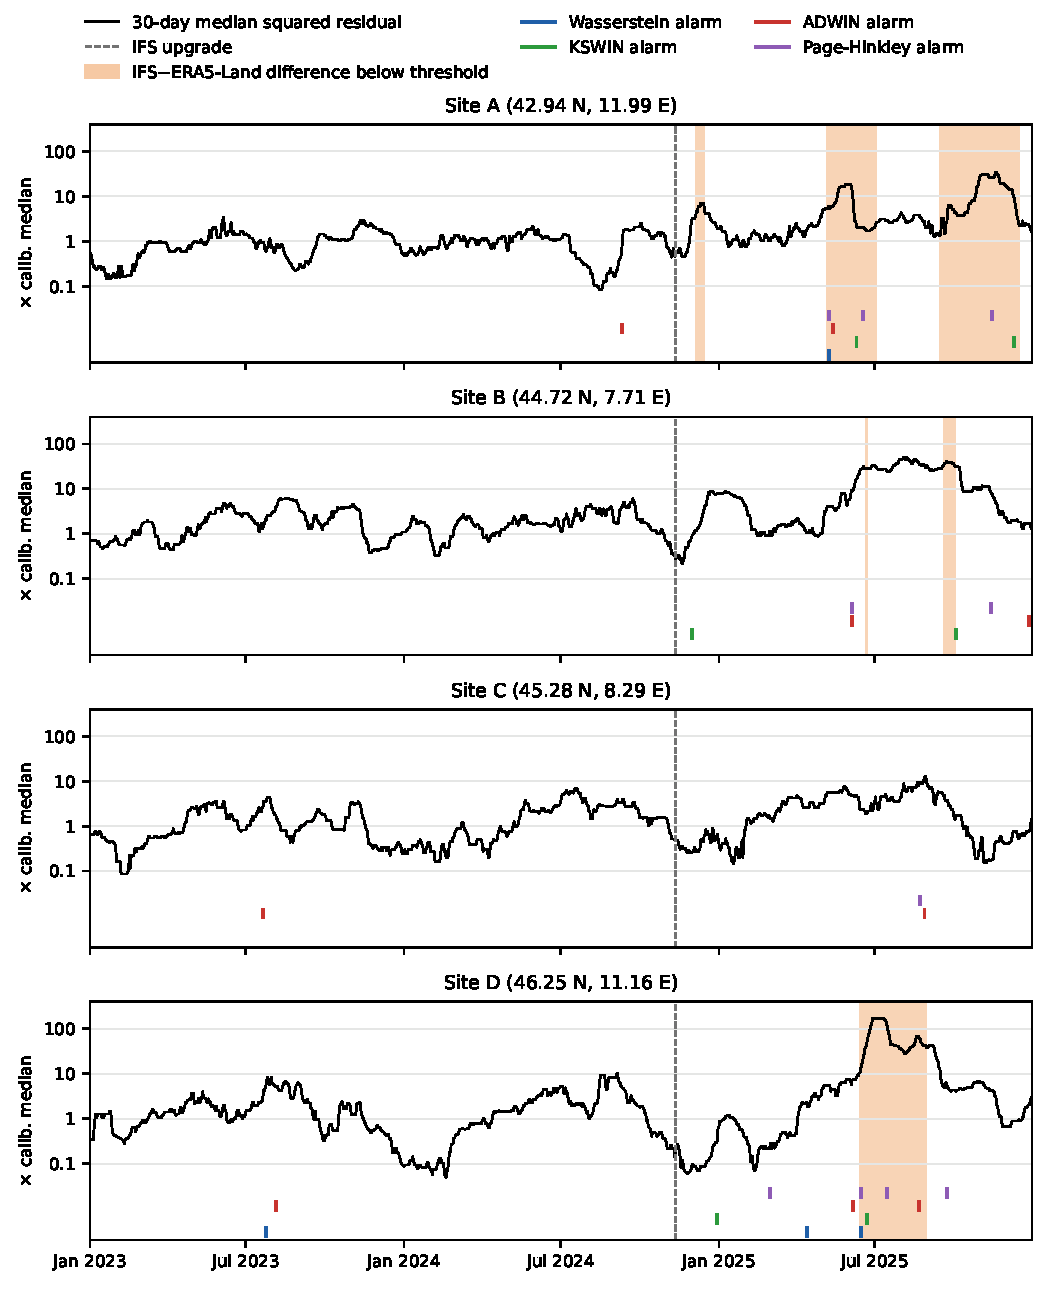
\includegraphics[width=\linewidth]{figures/soil_upstream_change.pdf}
\caption{Soil-moisture monitoring at the four sites. Black curves show the trailing 30-day median of daily squared residuals divided by the pooled calibration median, on a log scale. The dashed line marks the IFS upgrade. Shading identifies post-upgrade periods in which the smoothed IFS$-$ERA5-Land difference is below its episode threshold (Section~\ref{sec:soil-episodes}). Coloured ticks mark detector alarms on the IFS target, one row per detector.}\label{fig:soil}
\end{figure}


\section{Discussion and Limitations}
\label{sec:discussion}
\subsection{Main findings}
In the synthetic benchmark, the main strength of the Wasserstein detector is consistent coverage across change types. Its minimum observed excess detection over the seven scenarios is 0.90, while each baseline falls to placebo level in at least one scenario; within individual scenarios the leading detectors lie within sampling uncertainty of one another (Section~\ref{sec:coverage}). The contrast comes from the two scenarios that target a weakness of a mean-based or a Kolmogorov-Smirnov statistic, with squared residuals as the monitored signal, and applies to clearly separated mixture changes: at $\delta\leq0.70$ every detector stays at placebo level, and at $0.85$ the two distributional detectors detect about a third of the streams (Section~\ref{sec:severity}).

No detector is fastest everywhere. ADWIN has significantly shorter conditional delays on five functional changes, even though single misses on linear abrupt and F1$\to$F2 give it a worse capped mean there than Wasserstein. KSWIN detects the severe bimodal shift in about a quarter of Wasserstein's median delay and detects at least as often at every separation we tried. These rankings hold at the selected operating points (Section~\ref{sec:limitations}). Within the synthetic suite, ADWIN suits rapid detection of functional changes like ours, KSWIN noise-shape changes of the kind studied here, and Wasserstein a mix of the two types, where coverage across both matters more than speed. This guidance concerns single detectors. A combination of a mean-based detector and KSWIN, each given part of the budget, could also cover both blind regions identified here, and is a natural candidate for future comparison.

The results identify when a distributional detector is the better choice. Distributional monitoring is the better choice when the changes of concern may leave the mean of the monitored signal in place while moving its higher moments, since every signal admits such changes (Section~\ref{sec:coverage}). Within distributional monitoring, the Wasserstein distance is the better choice when a change may move a small share of the errors far, as on local drift, where the Kolmogorov-Smirnov statistic is capped by the affected mass (Eq.~\eqref{eq:mass}); for changes in the shape of the bulk of the distribution, KSWIN was at least as sensitive and faster. When the changes of concern move the mean and speed matters most, a mean-based detector such as ADWIN is preferable. Slow or incremental change lies outside the scope of these statements (Section~\ref{sec:limitations}); on real residuals, the soil-moisture case shows that the window and calibration design around the statistic also shape detector behaviour.

On real day-ahead residuals with a documented upstream change, Wasserstein raises the fewest alarms and stays within budget, and Page-Hinkley is the only detector whose alarm rate rises clearly more than on a control target. The real residuals are autocorrelated and can change gradually, unlike the abrupt i.i.d.\ changes of the benchmark, and a rolling reference adapts to such changes, as it did during the months-long rise in residuals at site B; a deployment that must flag persistent degradation can pair the detector with a fixed reference or a complementary monitor of the residual level. Which detector is preferable in a given deployment has to be checked on that deployment's data.

The ablations help explain where Wasserstein's coverage comes from. At matched calibration alarm rates, replacing the distance costs local-drift detection, while replacing the IQR bound or removing hysteresis costs bimodal detection. Hysteresis is a detector-agnostic alarm policy that could also reduce the baselines' repeated alarms. Coverage, by contrast, does not come from hysteresis alone: the KS variant keeps the same windows, IQR score and hysteresis, and still loses local-drift detection.

\subsection{Use as a prediction-system warning component}
\label{sec:operational}
The detector keeps prediction, monitoring and response apart. A fixed predictor supplies squared residuals as targets become available, the monitoring component turns them into alarms, and the application decides whether an alarm calls for investigation, uncertainty recalibration or retraining. A change in the error distribution does not by itself diagnose its cause or show that retraining will help. In the bimodal experiment expected squared loss is unchanged while the error distribution changes, so a trigger based on rising loss and a distributional warning answer different questions; the latter can still justify a closer look, or a recalibration of predictive uncertainty.

The operating choices we evaluated all involve trade-offs. A longer window accumulates more evidence but reacts later, hysteresis suppresses repeated alarms at the cost of missing a second change that arrives before re-arming, and batch-end testing changes score histories and calibrated parameters as well as latency. These choices should be checked on drift-free and changed streams from the application itself, with target availability counted in the response time. Calibration also needs enough drift-free data: with no calibration alarms at all, the Poisson upper bound of Eq.~\eqref{eq:ucb} falls to $0.1$ only after about 30,000 active samples, and the warm-up of about $3W$ residuals must be converted into time at the application's cadence.

The benchmark helps choose candidates for such a validation; demonstrating value at the system level would additionally require independently labelled operational events, a response rule, and measurements of prediction quality and intervention cost.

\subsection{Limitations}
\label{sec:limitations}
\paragraph{Calibration and operating points} All comparisons hold at the selected operating points. The common budget fixes a ceiling on the calibration bound, not a common realised false-alarm rate, and held-out null rates differ between detectors within a family, so speed rankings partly reflect how much of the budget each selection uses. The finite baseline searches cannot rule out other admissible operating points, and widened detectors receive more trials (80 instead of 40). The Poisson bound assumes an event-count model that overlapping windows and hysteresis do not guarantee, and trial selection reuses the calibration data, so the bound is a selection rule, not a distribution-free control of future false alarms: over the 80 repeated Wasserstein calibration draws, 12 held-out point estimates exceed the budget, and ADWIN's pre-change rates on the linear abrupt test streams at $B=50$ and $B=100$ are 0.105 and 0.107. Repeated calibration covers only Wasserstein and reuses the same test and null streams, so it does not show whether the ranking of detectors would survive recalibration of every detector, or whether batching changes the probability of exceeding the budget.

\paragraph{Ablations and batching} Ablation contrasts are made at recalibrated operating points, so they do not isolate a component at fixed parameters, and the no-hysteresis variant has zero placebo detection, so that comparison is not matched on held-out placebo rates. In the batch experiment, testing frequency, score histories and selected parameters change together, so their effects on delay cannot be separated; the experiment also aligns the change with the start of a complete batch.

\paragraph{Window selection} The false-alarm budget does not identify the window, since every tested window meets it with a suitable threshold. We fix the window by rule at the largest admissible value in the search range, so that the Wasserstein distance is estimated from as many reference samples as the protocol allows. This favours sensitivity to persistent shape changes over speed: at the same budget, smaller windows detect the functional changes slightly sooner. The rule and its range were fixed before any test stream was evaluated, and the cap of 1,000, which also equals the detection horizon, was set by the length of the streams (Section~\ref{sec:calibration}). Because every window is admissible, the rule always selects the cap, so the cap is in effect the window choice, and the bimodal detection rate of 0.98 reflects it; at $W=500$ it is 0.82 (Section~\ref{sec:sensitivity}).

\paragraph{Benchmark scope} The benchmark relies on synthetic generators, one fitted predictor per family and one change per stream, so its uncertainty reflects stream variability for that predictor only, and the coverage result is specific to these seven scenarios and change sizes. The suite contains no scenario aimed at a weakness of the Wasserstein detector, such as the slow or persistent change that a rolling reference absorbs (Section~\ref{sec:hysteresis}). The scenarios are constructions: the function switches stand for a change in the input--output relationship, such as a process or sensor recalibration, and the bimodal shift for a two-state disturbance at constant noise variance, but none is fitted to a documented production failure. Hysteresis was tested with one change per stream, so its effect on a second change that arrives before re-arming is unknown, and the suppression mechanism suggested for the threshold sweep (Section~\ref{sec:sensitivity}) was not checked stream by stream. Closely spaced changes, slow sustained evolution, delayed labels, serial dependence beyond these constructions, variation in model training and computational throughput remain to be evaluated.

\paragraph{Statistical inference} Paired tests are conditional on the fitted model and on a single calibration draw per detector. Wasserstein's held-out null rate varies from 0.040 to 0.112 across calibration draws (Tables~\ref{tab:robust} and~\ref{tab:batch-robust}), so the reported $p$-values, however small, do not include calibration variability. The explanations of the baselines' failures (Section~\ref{sec:coverage}) are population-level arguments: the KS bound concerns population distances, not the empirical statistic, and a mean-preserving change can still alter the finite-sample behaviour of mean-based detectors. Delay tests use only jointly detected streams, a non-significant result does not establish equivalence, and Wilson intervals are marginal, not simultaneous across scenarios. Differences from placebo and minima across scenarios are descriptive unless a test is reported, and ablation, sensitivity and capped-delay contrasts carry no multiplicity-adjusted inference. At $B=50$ and $B=100$ many delays on the strong functional changes tie at $B-1$, which reduces the information in delay tests and rankings.

\paragraph{Residual scale and outliers} Squaring amplifies large errors, and the Wasserstein distance responds to their magnitude; a quartile-based score does not make the detector robust to outliers in the original observations. Dividing ADWIN's and Page-Hinkley's unbounded inputs by the calibration median fixes their scale but does not bound ADWIN's inputs to $[0,1]$, so guarantees derived under other input assumptions do not automatically carry over. We provide no comparison matched on resources or computation.

\paragraph{Soil-moisture case} The case contains a single change event observed at four sites and is not designed as a statistical test. The episodes are defined from a second data product whose model differs from IFS, their boundaries depend on the smoothing window and percentile (\ref{app:soil-sensitivity}), and we did not check that each coincides with a change in the residual distribution. The placebo comparison of alarm timing involves only a handful of alarms. Calibration on two years of daily residuals admits only one or two alarms at the budget, and its transfer to autocorrelated residuals has not been assessed separately. The weather regressors, retrieved from the same archive, may themselves carry part of the upgrade.

\section{Conclusion}
\label{sec:conclusions}
We have compared ADWIN, KSWIN, Page-Hinkley and a calibrated Wasserstein detector on regression residuals, after calibrating all four to a common false-alarm budget on drift-free streams and auditing them on held-out null streams. Under this protocol the Wasserstein detector, which combines the empirical $1$-Wasserstein distance, a rolling IQR score and hysteresis, detects 96--100\% of streams in seven abrupt synthetic scenarios, while every baseline detects no more often than on null streams in one of the two scenarios built on a known weakness of its statistic. This holds for squared residuals and for the evaluated search ranges. The baselines lead on speed: ADWIN has shorter conditional delays on five functional changes, and KSWIN reacts sooner to the severe bimodal shift and detects weaker mixture changes at least as often. The ablations indicate that the distance, the IQR score and hysteresis all contribute at matched calibration alarm rates, and the detector keeps its high detection rates when residuals arrive in batches. Occasional held-out exceedances in the calibration studies show that the calibration criterion should be complemented by a held-out audit, as in our protocol. On an illustrative soil-moisture case, the Wasserstein detector raised the fewest alarms and stayed within its budget; its rolling reference adapted to a months-long rise in residuals at one site, so a deployment that must flag persistent degradation may pair it with a fixed-reference check of the residual level.

The results support distributional monitoring when the changes of concern may leave the mean of the monitored signal in place while moving its higher moments, and the Wasserstein distance in particular when a change may move a small share of the errors far. We recommend calibrating drift detectors to an explicit false-alarm budget before comparing them, with their realised held-out rates reported alongside. Future work should add slow and incremental changes to the benchmark, repeat calibration for every detector, evaluate the baselines on other residual transforms and with similar alarm suppression, and add real streams with documented changes and independently labelled operational events.

\section*{CRediT authorship contribution statement}
\textbf{Paolo Grazieschi:} Conceptualization, Methodology, Software, Formal analysis, Investigation, Writing -- original draft, Writing -- review \& editing, Visualization. \textbf{Romeo Silvestri:} Methodology, Software, Formal analysis, Investigation, Writing -- review \& editing.
\textbf{Massimo Vecchio:} Methodology, Supervision, Investigation, Writing -- review \& editing.
\textbf{Mattia Antonini:} Methodology, Investigation, Writing -- review \& editing.
\textbf{Fabio Antonelli:} Resources, Writing -- review \& editing.


\section*{Declaration of competing interest}
The authors declare that they have no known competing financial interests or personal relationships that could have appeared to influence the work reported in this paper.

\section*{Data availability}

This study uses synthetic data, generated as described in Section~\ref{sec:scenarios} and \ref{app:generators}, and soil-moisture, weather and weather-forecast series that are publicly available from the Open-Meteo historical archives. The code (BSD 3-Clause), retrieved series and outputs are publicly available in the \href{https://github.com/FBK-OpenIoT/calibrated-wasserstein-drift/releases/tag/v0.1.0}{v0.1.0 GitHub release}.

\section*{Funding}
This research did not receive any specific grant from funding agencies in the public, commercial, or not-for-profit sectors.

\section*{Declaration of generative AI and AI-assisted technologies in the manuscript preparation process}
During the preparation of this work the authors used Claude (Anthropic) to assist with manuscript restructuring, drafting, claim-consistency checks and LaTeX preparation. After using this tool, the authors reviewed and edited the content as needed and take full responsibility for the content of the published article.


\clearpage\appendix
\counterwithin*{table}{section}
\section{Generator Details}\label{app:generators}
Linear inputs are independent draws from $\mathcal U(0,1)^{10}$. The two weight vectors are independent uniform draws from $[-1,1]^{10}$ using one fixed weight-generator seed and are shared across streams. The bimodal construction uses the same input distribution and a single fixed weight vector throughout. These tests vary the sampled observations, not the underlying weight-vector draw.

For the five-feature function switches, the first function is
\begin{equation}
f_1(x)=10\sin(\pi x_0x_1)+20(x_2-0.5)^2+10x_3+5x_4.
\end{equation}
With $\omega(x_1)=40\pi+520\pi x_1$, define
\begin{align}
g_2(x)&=\sqrt{(100x_0)^2+\left(\omega(x_1)x_2-\frac{1}{\omega(x_1)(10x_3+1)}\right)^2}+5x_4,\\
f_2(x)&=(g_2(x)-482.13)\frac{4.882}{378.99}+14.414.
\end{align}
Inputs are uniform on $[0,1]^5$ and independent Gaussian noise has standard deviation 0.1. The affine constants are fixed generator values, not fitted on test outcomes. For the local and global Friedman scenarios, the change affects a restricted input region (LEA) or the regression function throughout the input space (GSG), respectively; the abrupt GSG case uses transition window zero. The monitoring index is offset from the generator's initial training segment so the first change is at monitoring index 15,000, and subsequent change points are placed outside the monitored interval.

\section{Selected Parameters}\label{app:parameters}
The three River Friedman scenarios share one calibration selection. Parameters are rounded for presentation.
\begingroup\small\setlength{\tabcolsep}{4pt}
\begin{longtable}{llrrr}
\caption{Selected main-benchmark parameters and calibration alarm rates per 1,000 active samples. Trials denotes the number of Optuna trials over all calibration rounds (40 per round); the Wasserstein window and threshold are computed exactly (Section~\ref{sec:calibration}). All configurations satisfy $U\leq0.1$; displayed values are rounded. ADWIN and Page-Hinkley parameters refer to squared errors divided by the family's calibration median (Section~\ref{sec:scenarios}). Widened range: ADWIN $\delta\in[10^{-9},0.1]$ on F1$\to$F2.}\label{tab:params}\\
\toprule
Detector & Parameters & Mean & UCB & Trials\\\midrule\endfirsthead
\multicolumn{5}{l}{\small Table \thetable\ continued}\\\toprule
Detector & Parameters & Mean & UCB & Trials\\\midrule\endhead
\bottomrule\endfoot
\multicolumn{5}{l}{\textit{Linear abrupt}}\\*
Wasserstein & $W=1000,\ \theta=1.7752$ & 0.071 & 0.099 & exact\\*
ADWIN & $\delta=0.004473$ & 0.070 & 0.096 & 40\\*
KSWIN & $W=700,\ \alpha=1.455\times10^{-4},\ m=46$ & 0.070 & 0.096 & 40\\*
Page-Hinkley & $\lambda=439.3118,\ \delta=0.001644$ & 0.070 & 0.096 & 40\\
\addlinespace
\multicolumn{5}{l}{\textit{F1$\to$F2}}\\*
Wasserstein & $W=1000,\ \theta=1.7330$ & 0.071 & 0.099 & exact\\*
ADWIN & $\delta=4.730\times10^{-6}$ & 0.068 & 0.093 & 80\\*
KSWIN & $W=575,\ \alpha=1.286\times10^{-4},\ m=36$ & 0.072 & 0.099 & 40\\*
Page-Hinkley & $\lambda=350.5906,\ \delta=0.1930$ & 0.058 & 0.082 & 40\\
\addlinespace
\multicolumn{5}{l}{\textit{F2$\to$F1}}\\*
Wasserstein & $W=1000,\ \theta=1.8262$ & 0.071 & 0.099 & exact\\*
ADWIN & $\delta=5.485\times10^{-4}$ & 0.073 & 0.099 & 40\\*
KSWIN & $W=695,\ \alpha=1.212\times10^{-4},\ m=54$ & 0.073 & 0.099 & 40\\*
Page-Hinkley & $\lambda=296.2705,\ \delta=0.1457$ & 0.068 & 0.093 & 40\\
\addlinespace
\multicolumn{5}{l}{\textit{River Friedman (shared)}}\\*
Wasserstein & $W=1000,\ \theta=1.9498$ & 0.071 & 0.099 & exact\\*
ADWIN & $\delta=4.996\times10^{-4}$ & 0.073 & 0.099 & 40\\*
KSWIN & $W=591,\ \alpha=8.179\times10^{-5},\ m=52$ & 0.070 & 0.096 & 40\\*
Page-Hinkley & $\lambda=445.3508,\ \delta=0.006014$ & 0.073 & 0.099 & 40\\
\addlinespace
\multicolumn{5}{l}{\textit{Bimodal shift}}\\*
Wasserstein & $W=1000,\ \theta=1.8915$ & 0.071 & 0.099 & exact\\*
ADWIN & $\delta=0.002622$ & 0.070 & 0.096 & 40\\*
KSWIN & $W=724,\ \alpha=1.407\times10^{-4},\ m=72$ & 0.070 & 0.097 & 40\\*
Page-Hinkley & $\lambda=418.6981,\ \delta=7.832\times10^{-5}$ & 0.073 & 0.099 & 40\\
\addlinespace
\end{longtable}\endgroup
\clearpage


\section{Additional Statistical Results}\label{app:statistics}
\begin{table}[htbp]\centering\small
\caption{Marginal 95\% Wilson intervals for all detection and placebo proportions appearing in Table~\ref{tab:main}, with 50 streams per estimate.}\label{tab:wilson}
\begin{tabular}{rrl}
\toprule
Alarmed horizons & Proportion & 95\% interval\\\midrule
0/50 & 0.00 & [0.000, 0.071]\\
1/50 & 0.02 & [0.004, 0.105]\\
2/50 & 0.04 & [0.011, 0.135]\\
3/50 & 0.06 & [0.021, 0.162]\\
4/50 & 0.08 & [0.032, 0.188]\\
5/50 & 0.10 & [0.043, 0.214]\\
6/50 & 0.12 & [0.056, 0.238]\\
47/50 & 0.94 & [0.838, 0.979]\\
48/50 & 0.96 & [0.865, 0.989]\\
49/50 & 0.98 & [0.895, 0.996]\\
50/50 & 1.00 & [0.929, 1.000]\\
\bottomrule\end{tabular}\end{table}

\begin{table}[htbp]\centering\small
\caption{The three significant main-benchmark detection contrasts. W-only and B-only count streams detected exclusively by Wasserstein or the baseline. Exact two-sided McNemar $p$-values are Holm-adjusted over all 21 scenario--baseline contrasts; all other adjusted values are 1.000.}\label{tab:mcnemar}
\setlength{\tabcolsep}{5pt}\begin{tabular}{llrrl}
\toprule
Scenario & Baseline & W-only & B-only & Adjusted $p$\\\midrule
Local abrupt (LEA) & KSWIN & 46 & 0 & $5.40\times10^{-13}$\\
Bimodal shift & ADWIN & 48 & 0 & $1.49\times10^{-13}$\\
Bimodal shift & Page-Hinkley & 48 & 0 & $1.49\times10^{-13}$\\
\bottomrule\end{tabular}\end{table}

\begingroup\small\setlength{\tabcolsep}{5pt}
\begin{longtable}{lrrll}
\caption{Paired conditional-delay comparisons against Wasserstein. The difference is baseline minus Wasserstein in samples, computed on jointly detected streams; it need not equal the difference between the full-sample medians in Table~\ref{tab:main}. Adjusted $p$ uses Holm correction over all 21 contrasts; n.s.\ denotes not significant. A dash suppresses comparisons for baselines failing the conditional-delay reporting rule, although their tests remain in the correction family.}\label{tab:paired}\\
\toprule
Baseline & Pairs & Median difference & Adjusted $p$ & Direction\\\midrule\endfirsthead
\multicolumn{5}{l}{\small Table \thetable\ continued}\\\toprule
Baseline & Pairs & Median difference & Adjusted $p$ & Direction\\\midrule\endhead
\bottomrule\endfoot
\multicolumn{5}{l}{\textit{Linear abrupt}}\\*
ADWIN & 49 & -2.0 & $6.05\times10^{-7}$ & Faster\\*
KSWIN & 47 & 20.0 & $3.21\times10^{-8}$ & Slower\\*
Page-Hinkley & 50 & 0.0 & 0.025 & Slower\\
\addlinespace
\multicolumn{5}{l}{\textit{F1$\to$F2}}\\*
ADWIN & 49 & -2.0 & $9.52\times10^{-7}$ & Faster\\*
KSWIN & 50 & 18.5 & $1.47\times10^{-8}$ & Slower\\*
Page-Hinkley & 50 & 0.0 & 0.092 & n.s.\\
\addlinespace
\multicolumn{5}{l}{\textit{F2$\to$F1}}\\*
ADWIN & 49 & 0.0 & 1.000 & n.s.\\*
KSWIN & 50 & 21.0 & $1.47\times10^{-8}$ & Slower\\*
Page-Hinkley & 50 & 0.0 & 1.000 & n.s.\\
\addlinespace
\multicolumn{5}{l}{\textit{Local abrupt (LEA)}}\\*
ADWIN & 47 & -56.0 & $1.71\times10^{-7}$ & Faster\\*
KSWIN & 2 & -- & -- & --\\*
Page-Hinkley & 48 & 0.0 & 1.000 & n.s.\\
\addlinespace
\multicolumn{5}{l}{\textit{Global abrupt (GSG)}}\\*
ADWIN & 49 & -8.0 & $2.10\times10^{-8}$ & Faster\\*
KSWIN & 49 & 21.0 & $2.10\times10^{-8}$ & Slower\\*
Page-Hinkley & 49 & 0.0 & 1.000 & n.s.\\
\addlinespace
\multicolumn{5}{l}{\textit{Transition 500}}\\*
ADWIN & 49 & -16.0 & $2.10\times10^{-8}$ & Faster\\*
KSWIN & 49 & 58.0 & $2.10\times10^{-8}$ & Slower\\*
Page-Hinkley & 49 & 0.0 & 0.544 & n.s.\\
\addlinespace
\multicolumn{5}{l}{\textit{Bimodal shift}}\\*
ADWIN & 1 & -- & -- & --\\*
KSWIN & 49 & -134.0 & $2.10\times10^{-8}$ & Faster\\*
Page-Hinkley & 1 & -- & -- & --\\
\addlinespace
\end{longtable}\endgroup\begin{table}[htbp]\centering\small
\caption{Per-scenario mean delay ranks with misses ranked worst (50 streams). All reported Holm-corrected omnibus tests reject. The Nemenyi critical difference is 0.830.}\label{tab:ranks}
\setlength{\tabcolsep}{4pt}\begin{tabular}{lrrrr}
\toprule
Scenario & Wasserstein & ADWIN & KSWIN & PH\\\midrule
Linear abrupt & 2.14 & 1.32 & 3.98 & 2.56\\
F1$\to$F2 & 2.44 & 1.41 & 3.98 & 2.17\\
F2$\to$F1 & 2.01 & 1.94 & 3.98 & 2.07\\
Local abrupt (LEA) & 2.42 & 1.30 & 3.97 & 2.31\\
Global abrupt (GSG) & 2.61 & 1.09 & 3.95 & 2.35\\
Transition 500 & 2.61 & 1.10 & 3.97 & 2.32\\
Bimodal shift & 2.02 & 3.49 & 1.00 & 3.49\\
\bottomrule\end{tabular}\end{table}
\clearpage
\section{Complete Ablation Results}\label{app:ablation}
Each variant is calibrated separately to the common false-alarm budget with the main benchmark's protocol; the full variant's rows therefore equal the Wasserstein rows of Table~\ref{tab:main}.
\begingroup\small\setlength{\tabcolsep}{4pt}
\begin{longtable}{lrrrrrr}
\caption{Ablation at a matched false-alarm budget, 50 test streams per scenario. Every variant is calibrated with the main benchmark's protocol: every selection uses $W=1000$, meets the budget and has the same calibration alarm rate, 0.071 per 1,000 active samples; $\theta$ is the selected threshold. Delays are among detected streams; n/a marks outcomes failing the conditional-delay reporting criterion. Flicker is per 1,000 post-change samples. The three River Friedman scenarios share one calibration per variant.}\label{tab:ablation}\\
\toprule
Variant & $\theta$ & Det. & Pl. & Median & Mean & Flicker\\\midrule\endfirsthead
\multicolumn{7}{l}{\small Table \thetable\ continued}\\\toprule
Variant & $\theta$ & Det. & Pl. & Median & Mean & Flicker\\\midrule\endhead
\bottomrule\endfoot
\multicolumn{7}{l}{\textit{Linear abrupt}}\\*
Full & 1.775 & 1.00 & 0.10 & 2.5 & 3.0 & 0.03\\*
No hysteresis & 6.084 & 1.00 & 0.00 & 5.0 & 5.3 & 110.20\\*
Mean/SD bound & 2.967 & 1.00 & 0.08 & 2.0 & 2.6 & 0.02\\*
KS statistic & 1.214 & 1.00 & 0.08 & 59.0 & 58.0 & 0.03\\*
Energy statistic & 1.784 & 1.00 & 0.10 & 12.0 & 12.6 & 0.02\\
\addlinespace
\multicolumn{7}{l}{\textit{F1$\to$F2}}\\*
Full & 1.733 & 1.00 & 0.08 & 3.5 & 4.1 & 0.02\\*
No hysteresis & 4.489 & 1.00 & 0.00 & 5.0 & 6.0 & 112.90\\*
Mean/SD bound & 2.740 & 0.98 & 0.10 & 2.0 & 3.3 & 0.04\\*
KS statistic & 1.310 & 1.00 & 0.08 & 57.5 & 60.8 & 0.00\\*
Energy statistic & 1.586 & 0.96 & 0.02 & 11.0 & 11.7 & 0.02\\
\addlinespace
\multicolumn{7}{l}{\textit{F2$\to$F1}}\\*
Full & 1.826 & 1.00 & 0.06 & 0.0 & 0.3 & 0.02\\*
No hysteresis & 4.191 & 1.00 & 0.00 & 0.0 & 0.3 & 114.30\\*
Mean/SD bound & 2.855 & 1.00 & 0.04 & 0.0 & 0.3 & 0.03\\*
KS statistic & 1.242 & 1.00 & 0.10 & 48.0 & 49.7 & 0.01\\*
Energy statistic & 1.618 & 1.00 & 0.14 & 1.0 & 1.5 & 0.02\\
\addlinespace
\multicolumn{7}{l}{\textit{Local abrupt (LEA)}}\\*
Full & 1.950 & 0.96 & 0.04 & 167.5 & 203.7 & 0.03\\*
No hysteresis & 4.821 & 0.88 & 0.00 & 257.5 & 257.6 & 56.56\\*
Mean/SD bound & 2.940 & 0.96 & 0.10 & 135.5 & 169.8 & 0.03\\*
KS statistic & 1.206 & 0.04 & 0.06 & n/a & n/a & 0.00\\*
Energy statistic & 1.614 & 0.34 & 0.02 & 427.0 & 471.3 & 0.02\\
\addlinespace
\multicolumn{7}{l}{\textit{Global abrupt (GSG)}}\\*
Full & 1.950 & 0.98 & 0.04 & 12.0 & 12.9 & 0.02\\*
No hysteresis & 4.821 & 1.00 & 0.00 & 17.0 & 19.0 & 110.40\\*
Mean/SD bound & 2.940 & 0.98 & 0.10 & 10.0 & 10.8 & 0.03\\*
KS statistic & 1.206 & 1.00 & 0.06 & 87.5 & 84.8 & 0.02\\*
Energy statistic & 1.614 & 0.96 & 0.02 & 30.0 & 30.5 & 0.02\\
\addlinespace
\multicolumn{7}{l}{\textit{Transition 500}}\\*
Full & 1.950 & 0.98 & 0.04 & 24.0 & 26.8 & 0.02\\*
No hysteresis & 4.821 & 1.00 & 0.00 & 37.5 & 39.6 & 109.10\\*
Mean/SD bound & 2.940 & 0.98 & 0.10 & 21.0 & 23.4 & 0.02\\*
KS statistic & 1.206 & 1.00 & 0.06 & 165.5 & 176.8 & 0.01\\*
Energy statistic & 1.614 & 0.98 & 0.02 & 58.0 & 62.2 & 0.01\\
\addlinespace
\multicolumn{7}{l}{\textit{Bimodal shift}}\\*
Full & 1.891 & 0.98 & 0.08 & 180.0 & 200.0 & 0.02\\*
No hysteresis & 4.959 & 0.74 & 0.00 & 288.0 & 297.4 & 39.57\\*
Mean/SD bound & 3.116 & 0.74 & 0.06 & 169.0 & 180.2 & 0.01\\*
KS statistic & 1.208 & 1.00 & 0.06 & 102.5 & 106.0 & 0.02\\*
Energy statistic & 1.619 & 1.00 & 0.10 & 142.0 & 148.5 & 0.02\\
\addlinespace
\end{longtable}\endgroup
\section{Complete Sensitivity Results}\label{app:sensitivity}
Settings marked $W^*$ or $\theta^*$ in the text are the calibrated values of each family. In the threshold sweep, calibrated thresholds are displayed as rounded values (e.g., 1.73 and 1.78), while evaluation uses the full-precision values.
\begingroup\small\setlength{\tabcolsep}{4pt}
\begin{longtable}{lrlrrrrl}
\caption{Sensitivity around the calibrated operating point, 50 test streams per setting. Window rows use the lowest threshold meeting the budget at that window (budget-matched); threshold rows hold the calibrated window $W^*=1000$; noise rows (linear abrupt) hold $W^*$ and re-match the threshold to calibration streams at each noise level. Delay is the median among detected streams. C-FP is the calibration alarm rate per 1,000 active samples; Budget uses the unrounded upper bound.}\label{tab:sensitivity}\\
\toprule
Factor & Value & Paired setting & Det. & Pl. & Delay & C-FP & Budget\\\midrule\endfirsthead
\multicolumn{8}{l}{\small Table \thetable\ continued}\\\toprule
Factor & Value & Paired setting & Det. & Pl. & Delay & C-FP & Budget\\\midrule\endhead
\bottomrule\endfoot
\multicolumn{8}{l}{\textit{Linear abrupt}}\\*
$W$ & 500 & $\theta=2.380$ & 1.00 & 0.00 & 2.0 & 0.070 & Yes\\*
$W$ & 600 & $\theta=2.341$ & 1.00 & 0.10 & 2.0 & 0.071 & Yes\\*
$W$ & 750 & $\theta=2.035$ & 1.00 & 0.10 & 2.0 & 0.070 & Yes\\*
$W$ & 900 & $\theta=2.059$ & 1.00 & 0.06 & 2.0 & 0.069 & Yes\\*
$W$ & 1000 & $\theta=1.775$ & 1.00 & 0.10 & 2.5 & 0.071 & Yes\\*
$\theta$ & 0 & $W=1000$ & 1.00 & 0.48 & 2.0 & 1.932 & No\\*
$\theta$ & 0.25 & $W=1000$ & 1.00 & 0.44 & 2.0 & 0.715 & No\\*
$\theta$ & 0.5 & $W=1000$ & 1.00 & 0.34 & 2.0 & 0.391 & No\\*
$\theta$ & 1 & $W=1000$ & 1.00 & 0.18 & 2.0 & 0.171 & No\\*
$\theta$ & 1.5 & $W=1000$ & 1.00 & 0.12 & 2.5 & 0.097 & No\\*
$\theta$ & 1.78 & $W=1000$ & 1.00 & 0.10 & 2.5 & 0.071 & Yes\\*
$\theta$ & 2 & $W=1000$ & 1.00 & 0.08 & 3.0 & 0.062 & Yes\\*
$\theta$ & 3 & $W=1000$ & 1.00 & 0.04 & 3.0 & 0.041 & Yes\\*
$\theta$ & 4 & $W=1000$ & 1.00 & 0.02 & 3.5 & 0.015 & Yes\\*
$\sigma$ & 0.05 & $W=1000,\ \theta=1.707$ & 1.00 & 0.12 & 2.0 & 0.071 & Yes\\*
$\sigma$ & 0.1 & $W=1000,\ \theta=1.775$ & 1.00 & 0.10 & 2.5 & 0.071 & Yes\\*
$\sigma$ & 0.2 & $W=1000,\ \theta=1.974$ & 1.00 & 0.14 & 6.0 & 0.071 & Yes\\*
$\sigma$ & 0.4 & $W=1000,\ \theta=1.857$ & 1.00 & 0.10 & 18.0 & 0.071 & Yes\\
\addlinespace
\multicolumn{8}{l}{\textit{F1$\to$F2}}\\*
$W$ & 500 & $\theta=2.812$ & 1.00 & 0.08 & 3.0 & 0.070 & Yes\\*
$W$ & 600 & $\theta=1.999$ & 1.00 & 0.14 & 2.0 & 0.071 & Yes\\*
$W$ & 750 & $\theta=1.696$ & 1.00 & 0.02 & 2.5 & 0.070 & Yes\\*
$W$ & 900 & $\theta=1.832$ & 1.00 & 0.08 & 2.5 & 0.069 & Yes\\*
$W$ & 1000 & $\theta=1.733$ & 1.00 & 0.08 & 3.5 & 0.071 & Yes\\*
$\theta$ & 0 & $W=1000$ & 0.96 & 0.40 & 2.0 & 1.462 & No\\*
$\theta$ & 0.25 & $W=1000$ & 0.96 & 0.28 & 2.0 & 0.600 & No\\*
$\theta$ & 0.5 & $W=1000$ & 0.96 & 0.24 & 2.0 & 0.353 & No\\*
$\theta$ & 1 & $W=1000$ & 0.98 & 0.16 & 2.0 & 0.194 & No\\*
$\theta$ & 1.5 & $W=1000$ & 1.00 & 0.12 & 3.0 & 0.091 & No\\*
$\theta$ & 1.73 & $W=1000$ & 1.00 & 0.08 & 3.5 & 0.071 & Yes\\*
$\theta$ & 2 & $W=1000$ & 1.00 & 0.06 & 3.5 & 0.041 & Yes\\*
$\theta$ & 3 & $W=1000$ & 1.00 & 0.04 & 4.0 & 0.026 & Yes\\*
$\theta$ & 4 & $W=1000$ & 1.00 & 0.00 & 4.0 & 0.012 & Yes\\
\addlinespace
\multicolumn{8}{l}{\textit{F2$\to$F1}}\\*
$W$ & 500 & $\theta=2.478$ & 0.98 & 0.00 & 0.0 & 0.070 & Yes\\*
$W$ & 600 & $\theta=2.173$ & 1.00 & 0.08 & 0.0 & 0.071 & Yes\\*
$W$ & 750 & $\theta=2.084$ & 1.00 & 0.06 & 0.0 & 0.070 & Yes\\*
$W$ & 900 & $\theta=1.820$ & 1.00 & 0.10 & 0.0 & 0.069 & Yes\\*
$W$ & 1000 & $\theta=1.826$ & 1.00 & 0.06 & 0.0 & 0.071 & Yes\\*
$\theta$ & 0 & $W=1000$ & 0.94 & 0.38 & 0.0 & 1.821 & No\\*
$\theta$ & 0.25 & $W=1000$ & 0.96 & 0.28 & 0.0 & 0.694 & No\\*
$\theta$ & 0.5 & $W=1000$ & 1.00 & 0.22 & 0.0 & 0.376 & No\\*
$\theta$ & 1 & $W=1000$ & 1.00 & 0.12 & 0.0 & 0.179 & No\\*
$\theta$ & 1.5 & $W=1000$ & 1.00 & 0.06 & 0.0 & 0.094 & No\\*
$\theta$ & 1.83 & $W=1000$ & 1.00 & 0.06 & 0.0 & 0.071 & Yes\\*
$\theta$ & 2 & $W=1000$ & 1.00 & 0.06 & 0.0 & 0.050 & Yes\\*
$\theta$ & 3 & $W=1000$ & 1.00 & 0.02 & 0.0 & 0.015 & Yes\\*
$\theta$ & 4 & $W=1000$ & 1.00 & 0.00 & 0.0 & 0.003 & Yes\\
\addlinespace
\multicolumn{8}{l}{\textit{Local abrupt (LEA)}}\\*
$W$ & 500 & $\theta=2.427$ & 0.98 & 0.06 & 135.0 & 0.070 & Yes\\*
$W$ & 600 & $\theta=2.173$ & 0.98 & 0.06 & 129.0 & 0.071 & Yes\\*
$W$ & 750 & $\theta=2.001$ & 0.98 & 0.06 & 145.0 & 0.070 & Yes\\*
$W$ & 900 & $\theta=2.006$ & 0.96 & 0.06 & 155.0 & 0.069 & Yes\\*
$W$ & 1000 & $\theta=1.950$ & 0.96 & 0.04 & 167.5 & 0.071 & Yes\\*
$\theta$ & 0 & $W=1000$ & 0.98 & 0.40 & 107.0 & 1.903 & No\\*
$\theta$ & 0.25 & $W=1000$ & 0.98 & 0.32 & 119.0 & 0.706 & No\\*
$\theta$ & 0.5 & $W=1000$ & 0.98 & 0.24 & 119.0 & 0.394 & No\\*
$\theta$ & 1 & $W=1000$ & 0.96 & 0.18 & 135.5 & 0.197 & No\\*
$\theta$ & 1.5 & $W=1000$ & 0.96 & 0.12 & 145.5 & 0.124 & No\\*
$\theta$ & 1.95 & $W=1000$ & 0.96 & 0.04 & 167.5 & 0.071 & Yes\\*
$\theta$ & 2 & $W=1000$ & 0.96 & 0.04 & 167.5 & 0.071 & Yes\\*
$\theta$ & 3 & $W=1000$ & 0.96 & 0.00 & 206.5 & 0.026 & Yes\\*
$\theta$ & 4 & $W=1000$ & 0.90 & 0.00 & 247.0 & 0.012 & Yes\\
\addlinespace
\multicolumn{8}{l}{\textit{Global abrupt (GSG)}}\\*
$W$ & 500 & $\theta=2.427$ & 1.00 & 0.06 & 10.0 & 0.070 & Yes\\*
$W$ & 600 & $\theta=2.173$ & 1.00 & 0.06 & 8.0 & 0.071 & Yes\\*
$W$ & 750 & $\theta=2.001$ & 1.00 & 0.06 & 10.0 & 0.070 & Yes\\*
$W$ & 900 & $\theta=2.006$ & 0.98 & 0.06 & 11.0 & 0.069 & Yes\\*
$W$ & 1000 & $\theta=1.950$ & 0.98 & 0.04 & 12.0 & 0.071 & Yes\\*
$\theta$ & 0 & $W=1000$ & 0.96 & 0.40 & 7.0 & 1.903 & No\\*
$\theta$ & 0.25 & $W=1000$ & 0.96 & 0.32 & 8.0 & 0.706 & No\\*
$\theta$ & 0.5 & $W=1000$ & 0.96 & 0.24 & 8.0 & 0.394 & No\\*
$\theta$ & 1 & $W=1000$ & 0.96 & 0.18 & 8.5 & 0.197 & No\\*
$\theta$ & 1.5 & $W=1000$ & 0.98 & 0.12 & 10.0 & 0.124 & No\\*
$\theta$ & 1.95 & $W=1000$ & 0.98 & 0.04 & 12.0 & 0.071 & Yes\\*
$\theta$ & 2 & $W=1000$ & 0.98 & 0.04 & 12.0 & 0.071 & Yes\\*
$\theta$ & 3 & $W=1000$ & 0.98 & 0.00 & 13.0 & 0.026 & Yes\\*
$\theta$ & 4 & $W=1000$ & 1.00 & 0.00 & 15.0 & 0.012 & Yes\\
\addlinespace
\multicolumn{8}{l}{\textit{Transition 500}}\\*
$W$ & 500 & $\theta=2.427$ & 1.00 & 0.06 & 21.0 & 0.070 & Yes\\*
$W$ & 600 & $\theta=2.173$ & 1.00 & 0.06 & 20.0 & 0.071 & Yes\\*
$W$ & 750 & $\theta=2.001$ & 1.00 & 0.06 & 22.0 & 0.070 & Yes\\*
$W$ & 900 & $\theta=2.006$ & 0.98 & 0.06 & 24.0 & 0.069 & Yes\\*
$W$ & 1000 & $\theta=1.950$ & 0.98 & 0.04 & 24.0 & 0.071 & Yes\\*
$\theta$ & 0 & $W=1000$ & 0.96 & 0.40 & 14.5 & 1.903 & No\\*
$\theta$ & 0.25 & $W=1000$ & 0.96 & 0.32 & 15.0 & 0.706 & No\\*
$\theta$ & 0.5 & $W=1000$ & 0.96 & 0.24 & 16.5 & 0.394 & No\\*
$\theta$ & 1 & $W=1000$ & 0.96 & 0.18 & 20.0 & 0.197 & No\\*
$\theta$ & 1.5 & $W=1000$ & 0.98 & 0.12 & 22.0 & 0.124 & No\\*
$\theta$ & 1.95 & $W=1000$ & 0.98 & 0.04 & 24.0 & 0.071 & Yes\\*
$\theta$ & 2 & $W=1000$ & 0.98 & 0.04 & 25.0 & 0.071 & Yes\\*
$\theta$ & 3 & $W=1000$ & 0.98 & 0.00 & 30.0 & 0.026 & Yes\\*
$\theta$ & 4 & $W=1000$ & 1.00 & 0.00 & 35.0 & 0.012 & Yes\\
\addlinespace
\multicolumn{8}{l}{\textit{Bimodal shift}}\\*
$W$ & 500 & $\theta=2.352$ & 0.82 & 0.04 & 166.0 & 0.070 & Yes\\*
$W$ & 600 & $\theta=2.244$ & 0.88 & 0.04 & 174.0 & 0.071 & Yes\\*
$W$ & 750 & $\theta=2.175$ & 0.94 & 0.06 & 170.0 & 0.070 & Yes\\*
$W$ & 900 & $\theta=2.171$ & 0.96 & 0.04 & 173.0 & 0.069 & Yes\\*
$W$ & 1000 & $\theta=1.891$ & 0.98 & 0.08 & 180.0 & 0.071 & Yes\\*
$\theta$ & 0 & $W=1000$ & 0.98 & 0.44 & 112.0 & 2.156 & No\\*
$\theta$ & 0.25 & $W=1000$ & 1.00 & 0.32 & 129.0 & 0.844 & No\\*
$\theta$ & 0.5 & $W=1000$ & 1.00 & 0.24 & 136.5 & 0.491 & No\\*
$\theta$ & 1 & $W=1000$ & 1.00 & 0.16 & 159.0 & 0.212 & No\\*
$\theta$ & 1.5 & $W=1000$ & 1.00 & 0.12 & 168.0 & 0.103 & No\\*
$\theta$ & 1.89 & $W=1000$ & 0.98 & 0.08 & 180.0 & 0.071 & Yes\\*
$\theta$ & 2 & $W=1000$ & 0.98 & 0.06 & 184.0 & 0.071 & Yes\\*
$\theta$ & 3 & $W=1000$ & 0.96 & 0.02 & 214.5 & 0.029 & Yes\\*
$\theta$ & 4 & $W=1000$ & 0.84 & 0.00 & 250.5 & 0.012 & Yes\\
\addlinespace
\end{longtable}\endgroup
\section{Batch-Size Calibration}\label{app:batch}
Each batch size is calibrated separately with the main benchmark's protocol (Section~\ref{sec:batches}); $B=1$ is Table~\ref{tab:params}. Parameters are rounded for presentation.
\begingroup\small\setlength{\tabcolsep}{2.5pt}
\begin{longtable}{rllrrrr}
\caption{Selected parameters for residuals in batches of $B$ samples. Mean and UCB are calibration alarm rates per 1,000 active samples; Null is the held-out null rate per 1,000 active samples. Trials counts Optuna trials over all calibration rounds (40 per round); the Wasserstein window and threshold are computed exactly. All configurations satisfy $U\leq0.1$; displayed values are rounded. PH denotes Page-Hinkley; ADWIN and PH parameters refer to the median-normalised signal. Widened ranges: ADWIN $\delta\in[10^{-5},0.999]$ on linear abrupt at $B=100$; KSWIN window size $\in[50,1000]$ on River Friedman at $B=50$ and on F1$\to$F2 at $B=100$, and KSWIN $\alpha\in[10^{-5},0.5]$ on F1$\to$F2, F2$\to$F1 and River Friedman at $B=100$.}\label{tab:batch-params}\\
\toprule
$B$ & Detector & Parameters & Mean & UCB & Null & Trials\\\midrule\endfirsthead
\multicolumn{7}{l}{\small Table \thetable\ continued}\\\toprule
$B$ & Detector & Parameters & Mean & UCB & Null & Trials\\\midrule\endhead
\bottomrule\endfoot
\multicolumn{7}{l}{\textit{Linear abrupt}}\\*
10 & Wasserstein & $W=1000,\ \theta=1.6423$ & 0.071 & 0.099 & 0.064 & exact \\*
10 & ADWIN & $\delta=0.009393$ & 0.070 & 0.096 & 0.052 & 40 \\*
10 & KSWIN & $W=920,\ \alpha=0.001329,\ m=47$ & 0.063 & 0.088 & 0.077 & 40 \\*
10 & PH & $\lambda=439.3,\ \delta=0.001644$ & 0.073 & 0.099 & 0.065 & 40 \\*
50 & Wasserstein & $W=1000,\ \theta=1.6515$ & 0.071 & 0.099 & 0.051 & exact \\*
50 & ADWIN & $\delta=0.04730$ & 0.073 & 0.099 & 0.078 & 40 \\*
50 & KSWIN & $W=511,\ \alpha=0.006144,\ m=42$ & 0.072 & 0.099 & 0.081 & 40 \\*
50 & PH & $\lambda=422.3,\ \delta=0.001960$ & 0.073 & 0.099 & 0.064 & 40 \\*
100 & Wasserstein & $W=1000,\ \theta=1.7927$ & 0.071 & 0.099 & 0.047 & exact \\*
100 & ADWIN & $\delta=0.08885$ & 0.070 & 0.096 & 0.088 & 80 \\*
100 & KSWIN & $W=531,\ \alpha=0.008205,\ m=77$ & 0.067 & 0.093 & 0.062 & 40 \\*
100 & PH & $\lambda=453.4,\ \delta=6.493\times10^{-4}$ & 0.065 & 0.091 & 0.058 & 40 \\
\addlinespace
\multicolumn{7}{l}{\textit{F1$\to$F2}}\\*
10 & Wasserstein & $W=1000,\ \theta=1.6702$ & 0.071 & 0.099 & 0.068 & exact \\*
10 & ADWIN & $\delta=6.704\times10^{-5}$ & 0.073 & 0.099 & 0.087 & 40 \\*
10 & KSWIN & $W=870,\ \alpha=8.496\times10^{-4},\ m=46$ & 0.065 & 0.091 & 0.053 & 40 \\*
10 & PH & $\lambda=176.3,\ \delta=0.7649$ & 0.073 & 0.099 & 0.074 & 40 \\*
50 & Wasserstein & $W=1000,\ \theta=1.7268$ & 0.071 & 0.099 & 0.058 & exact \\*
50 & ADWIN & $\delta=0.001556$ & 0.073 & 0.099 & 0.094 & 40 \\*
50 & KSWIN & $W=564,\ \alpha=0.004317,\ m=51$ & 0.072 & 0.099 & 0.045 & 40 \\*
50 & PH & $\lambda=294.4,\ \delta=0.2114$ & 0.073 & 0.099 & 0.079 & 40 \\*
100 & Wasserstein & $W=1000,\ \theta=1.3880$ & 0.071 & 0.099 & 0.092 & exact \\*
100 & ADWIN & $\delta=0.004666$ & 0.070 & 0.096 & 0.075 & 40 \\*
100 & KSWIN & $W=502,\ \alpha=0.00972,\ m=67$ & 0.070 & 0.096 & 0.065 & 80 \\*
100 & PH & $\lambda=402.3,\ \delta=0.08066$ & 0.073 & 0.099 & 0.085 & 40 \\
\addlinespace
\multicolumn{7}{l}{\textit{F2$\to$F1}}\\*
10 & Wasserstein & $W=1000,\ \theta=1.6889$ & 0.071 & 0.099 & 0.080 & exact \\*
10 & ADWIN & $\delta=0.001707$ & 0.068 & 0.093 & 0.074 & 40 \\*
10 & KSWIN & $W=678,\ \alpha=0.001027,\ m=47$ & 0.067 & 0.093 & 0.089 & 40 \\*
10 & PH & $\lambda=296.3,\ \delta=0.1457$ & 0.065 & 0.090 & 0.068 & 40 \\*
50 & Wasserstein & $W=1000,\ \theta=1.6875$ & 0.071 & 0.099 & 0.062 & exact \\*
50 & ADWIN & $\delta=0.009182$ & 0.073 & 0.099 & 0.054 & 40 \\*
50 & KSWIN & $W=592,\ \alpha=0.002938,\ m=74$ & 0.067 & 0.093 & 0.063 & 40 \\*
50 & PH & $\lambda=320.5,\ \delta=0.1085$ & 0.073 & 0.099 & 0.065 & 40 \\*
100 & Wasserstein & $W=1000,\ \theta=1.6590$ & 0.071 & 0.099 & 0.071 & exact \\*
100 & ADWIN & $\delta=0.02178$ & 0.068 & 0.094 & 0.066 & 40 \\*
100 & KSWIN & $W=673,\ \alpha=0.009716,\ m=67$ & 0.073 & 0.099 & 0.086 & 80 \\*
100 & PH & $\lambda=320.5,\ \delta=0.1085$ & 0.065 & 0.091 & 0.062 & 40 \\
\addlinespace
\multicolumn{7}{l}{\textit{River Friedman (shared)}}\\*
10 & Wasserstein & $W=1000,\ \theta=1.9081$ & 0.071 & 0.099 & 0.054 & exact \\*
10 & ADWIN & $\delta=9.576\times10^{-4}$ & 0.065 & 0.090 & 0.072 & 40 \\*
10 & KSWIN & $W=841,\ \alpha=0.001391,\ m=41$ & 0.070 & 0.097 & 0.066 & 40 \\*
10 & PH & $\lambda=59.26,\ \delta=3.369$ & 0.073 & 0.099 & 0.074 & 40 \\*
50 & Wasserstein & $W=1000,\ \theta=1.6483$ & 0.071 & 0.099 & 0.062 & exact \\*
50 & ADWIN & $\delta=0.01477$ & 0.073 & 0.099 & 0.093 & 40 \\*
50 & KSWIN & $W=164,\ \alpha=0.004106,\ m=36$ & 0.073 & 0.100 & 0.076 & 80 \\*
50 & PH & $\lambda=431.1,\ \delta=0.008606$ & 0.070 & 0.096 & 0.074 & 40 \\*
100 & Wasserstein & $W=1000,\ \theta=1.8603$ & 0.071 & 0.099 & 0.066 & exact \\*
100 & ADWIN & $\delta=0.03400$ & 0.065 & 0.091 & 0.084 & 40 \\*
100 & KSWIN & $W=599,\ \alpha=0.009626,\ m=63$ & 0.072 & 0.099 & 0.051 & 80 \\*
100 & PH & $\lambda=400.0,\ \delta=0.01885$ & 0.073 & 0.099 & 0.069 & 40 \\
\addlinespace
\multicolumn{7}{l}{\textit{Bimodal shift}}\\*
10 & Wasserstein & $W=1000,\ \theta=1.7159$ & 0.071 & 0.099 & 0.072 & exact \\*
10 & ADWIN & $\delta=0.005085$ & 0.065 & 0.090 & 0.056 & 40 \\*
10 & KSWIN & $W=905,\ \alpha=0.001161,\ m=36$ & 0.071 & 0.098 & 0.049 & 40 \\*
10 & PH & $\lambda=407.9,\ \delta=0.002267$ & 0.073 & 0.099 & 0.071 & 40 \\*
50 & Wasserstein & $W=1000,\ \theta=1.2361$ & 0.071 & 0.099 & 0.105 & exact \\*
50 & ADWIN & $\delta=0.01849$ & 0.063 & 0.088 & 0.043 & 40 \\*
50 & KSWIN & $W=559,\ \alpha=0.003475,\ m=46$ & 0.070 & 0.096 & 0.061 & 40 \\*
50 & PH & $\lambda=404.4,\ \delta=0.003680$ & 0.073 & 0.099 & 0.065 & 40 \\*
100 & Wasserstein & $W=1000,\ \theta=1.7124$ & 0.071 & 0.099 & 0.076 & exact \\*
100 & ADWIN & $\delta=0.05402$ & 0.073 & 0.099 & 0.057 & 40 \\*
100 & KSWIN & $W=687,\ \alpha=0.007114,\ m=64$ & 0.070 & 0.096 & 0.060 & 40 \\*
100 & PH & $\lambda=389.7,\ \delta=0.006876$ & 0.070 & 0.096 & 0.065 & 40 \\
\addlinespace
\end{longtable}\endgroup


\section{Sensitivity of soil-case episode scoring}
\label{app:soil-sensitivity}
We recompute the episodes from the saved hourly IFS and ERA5-Land series, first averaging the difference per day and then applying a trailing mean. Each site's threshold is the specified percentile of the smoothed difference over 1 January 2021--11 November 2024, with linear percentile interpolation. Episodes are evaluated from 12 November 2024 to 30 December 2025; a new episode starts at a below-threshold day only if more than 30 days have elapsed since the preceding below-threshold day. This separation rule is held fixed across the grid. Detectors, parameters and alarm sequences are unchanged. Primary scoring counts an episode as detected if an alarm falls in the inclusive interval from its start to 42 days afterwards, restricted to the post-upgrade monitoring period.

\begin{table}[htbp]\centering\small
\caption{Sensitivity to the episode definition, using the primary 0--42-day alarm-matching window. $L$ is the smoothing window in days and $p$ the pre-upgrade percentile. The four rightmost columns count detected episodes, with the total in the Episodes column. W denotes Wasserstein and PH Page-Hinkley. The main definition is $L=30$, $p=1$.}\label{tab:soil-sensitivity}
\setlength{\tabcolsep}{5pt}
\begin{tabular}{rrrrrrrr}
\toprule
$L$ & $p$ & Episodes & Sites & W & KSWIN & ADWIN & PH\\\midrule
15 & 0.5 & 7 & ABCD & 2 & 3 & 2 & 3\\
15 & 1.0 & 7 & ABCD & 2 & 3 & 2 & 3\\
15 & 2.0 & 8 & ABCD & 2 & 3 & 2 & 3\\
30 & 0.5 & 5 & ABD & 2 & 3 & 1 & 2\\
30 & 1.0 & 6 & ABD & 2 & 3 & 1 & 2\\
30 & 2.0 & 6 & ABD & 2 & 3 & 1 & 2\\
60 & 0.5 & 4 & ABD & 0 & 2 & 1 & 3\\
60 & 1.0 & 4 & ABD & 0 & 2 & 1 & 3\\
60 & 2.0 & 4 & ABD & 0 & 2 & 1 & 3\\
\bottomrule
\end{tabular}
\end{table}

With primary scoring, Wasserstein detects two episodes at the 15- and 30-day smoothing windows and none at the 60-day window. KSWIN detects two to three, ADWIN one to two, and Page-Hinkley two to three. Both the episode denominator and the detected counts therefore depend on the episode definition.

With the main six episodes held fixed, we separately vary the alarm-matching lead over 0, 15 and 30 days and the lag over 14, 42 and 90 days. Wasserstein detects two throughout; KSWIN detects one to four, ADWIN one to three, and Page-Hinkley two to five. The primary 0--42-day window gives two detections for Wasserstein and Page-Hinkley, three for KSWIN and one for ADWIN. Allowing a 30-day lead with the same 42-day lag gives two, three, three and three, respectively. This lead allows for the lag of the trailing mean used to define episodes, but can also credit unrelated earlier alarms; it is retained only as a sensitivity check. All matching windows are clipped at the upgrade date and monitoring end. These post-hoc checks show how the counts depend on scoring choices.

\begingroup\small
\setlength{\bibsep}{4pt plus 1pt minus 1pt}
\bibliographystyle{elsarticle-num}
\bibliography{references}
\endgroup

\end{document}
